\documentclass[]{article}
\usepackage{lmodern}
\usepackage{amssymb,amsmath}
\usepackage{ifxetex,ifluatex}
\usepackage{fixltx2e} % provides \textsubscript
\ifnum 0\ifxetex 1\fi\ifluatex 1\fi=0 % if pdftex
  \usepackage[T1]{fontenc}
  \usepackage[utf8]{inputenc}
\else % if luatex or xelatex
  \ifxetex
    \usepackage{mathspec}
  \else
    \usepackage{fontspec}
  \fi
  \defaultfontfeatures{Ligatures=TeX,Scale=MatchLowercase}
\fi
% use upquote if available, for straight quotes in verbatim environments
\IfFileExists{upquote.sty}{\usepackage{upquote}}{}
% use microtype if available
\IfFileExists{microtype.sty}{%
\usepackage[]{microtype}
\UseMicrotypeSet[protrusion]{basicmath} % disable protrusion for tt fonts
}{}
\PassOptionsToPackage{hyphens}{url} % url is loaded by hyperref
\usepackage[unicode=true]{hyperref}
\hypersetup{
            pdftitle={A correlation analysis of clinical variables of TCGA-KIRC patients},
            pdfborder={0 0 0},
            breaklinks=true}
\urlstyle{same}  % don't use monospace font for urls
\usepackage[margin=1in]{geometry}
\usepackage{color}
\usepackage{fancyvrb}
\newcommand{\VerbBar}{|}
\newcommand{\VERB}{\Verb[commandchars=\\\{\}]}
\DefineVerbatimEnvironment{Highlighting}{Verbatim}{commandchars=\\\{\}}
% Add ',fontsize=\small' for more characters per line
\usepackage{framed}
\definecolor{shadecolor}{RGB}{248,248,248}
\newenvironment{Shaded}{\begin{snugshade}}{\end{snugshade}}
\newcommand{\KeywordTok}[1]{\textcolor[rgb]{0.13,0.29,0.53}{\textbf{#1}}}
\newcommand{\DataTypeTok}[1]{\textcolor[rgb]{0.13,0.29,0.53}{#1}}
\newcommand{\DecValTok}[1]{\textcolor[rgb]{0.00,0.00,0.81}{#1}}
\newcommand{\BaseNTok}[1]{\textcolor[rgb]{0.00,0.00,0.81}{#1}}
\newcommand{\FloatTok}[1]{\textcolor[rgb]{0.00,0.00,0.81}{#1}}
\newcommand{\ConstantTok}[1]{\textcolor[rgb]{0.00,0.00,0.00}{#1}}
\newcommand{\CharTok}[1]{\textcolor[rgb]{0.31,0.60,0.02}{#1}}
\newcommand{\SpecialCharTok}[1]{\textcolor[rgb]{0.00,0.00,0.00}{#1}}
\newcommand{\StringTok}[1]{\textcolor[rgb]{0.31,0.60,0.02}{#1}}
\newcommand{\VerbatimStringTok}[1]{\textcolor[rgb]{0.31,0.60,0.02}{#1}}
\newcommand{\SpecialStringTok}[1]{\textcolor[rgb]{0.31,0.60,0.02}{#1}}
\newcommand{\ImportTok}[1]{#1}
\newcommand{\CommentTok}[1]{\textcolor[rgb]{0.56,0.35,0.01}{\textit{#1}}}
\newcommand{\DocumentationTok}[1]{\textcolor[rgb]{0.56,0.35,0.01}{\textbf{\textit{#1}}}}
\newcommand{\AnnotationTok}[1]{\textcolor[rgb]{0.56,0.35,0.01}{\textbf{\textit{#1}}}}
\newcommand{\CommentVarTok}[1]{\textcolor[rgb]{0.56,0.35,0.01}{\textbf{\textit{#1}}}}
\newcommand{\OtherTok}[1]{\textcolor[rgb]{0.56,0.35,0.01}{#1}}
\newcommand{\FunctionTok}[1]{\textcolor[rgb]{0.00,0.00,0.00}{#1}}
\newcommand{\VariableTok}[1]{\textcolor[rgb]{0.00,0.00,0.00}{#1}}
\newcommand{\ControlFlowTok}[1]{\textcolor[rgb]{0.13,0.29,0.53}{\textbf{#1}}}
\newcommand{\OperatorTok}[1]{\textcolor[rgb]{0.81,0.36,0.00}{\textbf{#1}}}
\newcommand{\BuiltInTok}[1]{#1}
\newcommand{\ExtensionTok}[1]{#1}
\newcommand{\PreprocessorTok}[1]{\textcolor[rgb]{0.56,0.35,0.01}{\textit{#1}}}
\newcommand{\AttributeTok}[1]{\textcolor[rgb]{0.77,0.63,0.00}{#1}}
\newcommand{\RegionMarkerTok}[1]{#1}
\newcommand{\InformationTok}[1]{\textcolor[rgb]{0.56,0.35,0.01}{\textbf{\textit{#1}}}}
\newcommand{\WarningTok}[1]{\textcolor[rgb]{0.56,0.35,0.01}{\textbf{\textit{#1}}}}
\newcommand{\AlertTok}[1]{\textcolor[rgb]{0.94,0.16,0.16}{#1}}
\newcommand{\ErrorTok}[1]{\textcolor[rgb]{0.64,0.00,0.00}{\textbf{#1}}}
\newcommand{\NormalTok}[1]{#1}
\usepackage{longtable,booktabs}
% Fix footnotes in tables (requires footnote package)
\IfFileExists{footnote.sty}{\usepackage{footnote}\makesavenoteenv{long table}}{}
\usepackage{graphicx,grffile}
\makeatletter
\def\maxwidth{\ifdim\Gin@nat@width>\linewidth\linewidth\else\Gin@nat@width\fi}
\def\maxheight{\ifdim\Gin@nat@height>\textheight\textheight\else\Gin@nat@height\fi}
\makeatother
% Scale images if necessary, so that they will not overflow the page
% margins by default, and it is still possible to overwrite the defaults
% using explicit options in \includegraphics[width, height, ...]{}
\setkeys{Gin}{width=\maxwidth,height=\maxheight,keepaspectratio}
\IfFileExists{parskip.sty}{%
\usepackage{parskip}
}{% else
\setlength{\parindent}{0pt}
\setlength{\parskip}{6pt plus 2pt minus 1pt}
}
\setlength{\emergencystretch}{3em}  % prevent overfull lines
\providecommand{\tightlist}{%
  \setlength{\itemsep}{0pt}\setlength{\parskip}{0pt}}
\setcounter{secnumdepth}{0}
% Redefines (sub)paragraphs to behave more like sections
\ifx\paragraph\undefined\else
\let\oldparagraph\paragraph
\renewcommand{\paragraph}[1]{\oldparagraph{#1}\mbox{}}
\fi
\ifx\subparagraph\undefined\else
\let\oldsubparagraph\subparagraph
\renewcommand{\subparagraph}[1]{\oldsubparagraph{#1}\mbox{}}
\fi

% set default figure placement to htbp
\makeatletter
\def\fps@figure{htbp}
\makeatother


\title{A correlation analysis of clinical variables of TCGA-KIRC patients}
\author{}
\date{\vspace{-2.5em}}

\begin{document}
\maketitle

This project contains a pipeline of clinical analysis of the Cancer
Genome Atlas Kidney Renal Clear Cell Carcinoma (TCGA-KIRC) data of
patients, from
\href{https://portal.gdc.cancer.gov/exploration?filters=\%7B\%22op\%22\%3A\%22and\%22\%2C\%22content\%22\%3A\%5B\%7B\%22op\%22\%3A\%22in\%22\%2C\%22content\%22\%3A\%7B\%22field\%22\%3A\%22cases.project.project_id\%22\%2C\%22value\%22\%3A\%5B\%22TCGA-KIRC\%22\%5D\%7D\%7D\%5D\%7D}{Genomic
Data Commons Data Portal} and
\href{https://www.cbioportal.org/study/summary?id=kirp_tcga}{cBioPortal}.

Previously, we presented \href{1.preprocessing.md}{an exploratory
preprocessing analysis}. In this section, Chi-squared test is applied to
compare two or more proportions of categorical variables and T-student
test to compare the means of numeric ones regardind the levels of
`Overall\_Survival\_Status'. The Hypoteis test is performed and p-value
indicates the strength of evidence in supportting the null hypothesis.

\begin{Shaded}
\begin{Highlighting}[]
\CommentTok{# Set the packages of interest}
\NormalTok{packages =}\StringTok{ }\KeywordTok{c}\NormalTok{(}\StringTok{"tidyverse"}\NormalTok{,}\StringTok{"skimr"}\NormalTok{,}\StringTok{"finalfit"}\NormalTok{,}\StringTok{"rstatix"}\NormalTok{, }\StringTok{"ggpubr"}\NormalTok{,}\StringTok{"GGally"}\NormalTok{)}

\CommentTok{# if a package is installed, it will be loaded}
\CommentTok{# otherwise, the missing package(s) will be installed and loaded}
\NormalTok{package.check <-}\StringTok{ }\KeywordTok{lapply}\NormalTok{(packages, }\DataTypeTok{FUN =} \ControlFlowTok{function}\NormalTok{(x) \{}
  \ControlFlowTok{if}\NormalTok{ (}\OperatorTok{!}\KeywordTok{require}\NormalTok{(x, }\DataTypeTok{character.only =} \OtherTok{TRUE}\NormalTok{)) \{}
    \KeywordTok{install.packages}\NormalTok{(x, }\DataTypeTok{dependencies =} \OtherTok{TRUE}\NormalTok{)}
    \KeywordTok{library}\NormalTok{(x, }\DataTypeTok{character.only =} \OtherTok{TRUE}\NormalTok{)}
\NormalTok{  \}}
\NormalTok{\})}

\KeywordTok{suppressMessages}\NormalTok{(}\KeywordTok{library}\NormalTok{(}\StringTok{"tidyverse"}\NormalTok{))}
\KeywordTok{setwd}\NormalTok{(}\StringTok{"."}\NormalTok{)}
\end{Highlighting}
\end{Shaded}

\subsection{1. Importing data}\label{importing-data}

\begin{Shaded}
\begin{Highlighting}[]
\NormalTok{kirc_clinic <-}\StringTok{ }\KeywordTok{read_csv}\NormalTok{(}\StringTok{"data/kirc_clinic.csv"}\NormalTok{)}
\end{Highlighting}
\end{Shaded}

\subsection{2. Taming data}\label{taming-data}

\begin{Shaded}
\begin{Highlighting}[]
\NormalTok{kirc_clinic <-}\StringTok{ }\NormalTok{kirc_clinic }\OperatorTok
\StringTok{  }\KeywordTok{mutate_if}\NormalTok{(is.character, as.factor) }\OperatorTok
\StringTok{  }\KeywordTok{mutate}\NormalTok{(}\DataTypeTok{patient_id =} \KeywordTok{as.character}\NormalTok{(patient_id))}
\end{Highlighting}
\end{Shaded}

\subsection{3. Checking variables}\label{checking-variables}

\begin{Shaded}
\begin{Highlighting}[]
\KeywordTok{skim}\NormalTok{(kirc_clinic) }
\end{Highlighting}
\end{Shaded}

\begin{longtable}[]{@{}ll@{}}
\caption{Data summary}\tabularnewline
\toprule
Name & kirc\_clinic\tabularnewline
Number of rows & 537\tabularnewline
Number of columns & 32\tabularnewline
\_\_\_\_\_\_\_\_\_\_\_\_\_\_\_\_\_\_\_\_\_\_\_ &\tabularnewline
Column type frequency: &\tabularnewline
character & 1\tabularnewline
factor & 22\tabularnewline
numeric & 9\tabularnewline
\_\_\_\_\_\_\_\_\_\_\_\_\_\_\_\_\_\_\_\_\_\_\_\_ &\tabularnewline
Group variables & None\tabularnewline
\bottomrule
\end{longtable}

\textbf{Variable type: character}

\begin{longtable}[]{@{}lrrrrrrr@{}}
\toprule
skim\_variable & n\_missing & complete\_rate & min & max & empty &
n\_unique & whitespace\tabularnewline
\midrule
\endhead
patient\_id & 0 & 1 & 12 & 12 & 0 & 537 & 0\tabularnewline
\bottomrule
\end{longtable}

\textbf{Variable type: factor}

\begin{longtable}[]{@{}lrrlrl@{}}
\toprule
skim\_variable & n\_missing & complete\_rate & ordered & n\_unique &
top\_counts\tabularnewline
\midrule
\endhead
metastasis\_stg & 2 & 1.00 & FALSE & 3 & M0: 426, M1: 79, MX:
30\tabularnewline
neoplasm\_ln\_stg & 0 & 1.00 & FALSE & 3 & NX: 280, N0: 240, N1:
17\tabularnewline
neoplasm\_stg & 3 & 0.99 & FALSE & 4 & Sta: 269, Sta: 125, Sta: 83, Sta:
57\tabularnewline
tumor\_stg & 0 & 1.00 & FALSE & 4 & T1: 275, T3: 182, T2: 69, T4:
11\tabularnewline
disease\_free\_stt & 99 & 0.82 & FALSE & 2 & Dis: 311, Rec:
127\tabularnewline
ethnicity & 152 & 0.72 & FALSE & 2 & NOT: 359, HIS: 26\tabularnewline
histology\_grd & 3 & 0.99 & FALSE & 5 & G2: 230, G3: 207, G4: 78, G1:
14\tabularnewline
hemoglobin & 83 & 0.85 & FALSE & 3 & Low: 263, Nor: 186, Ele:
5\tabularnewline
neoadj\_therapy & 0 & 1.00 & FALSE & 2 & No: 519, Yes: 18\tabularnewline
prior\_cancer & 0 & 1.00 & FALSE & 2 & No: 459, Yes: 78\tabularnewline
tumor\_lateral & 0 & 1.00 & FALSE & 3 & Rig: 283, Lef: 253, Bil:
1\tabularnewline
primer\_ln\_ind3 & 7 & 0.99 & FALSE & 2 & NO: 395, YES:
135\tabularnewline
over\_surv\_stt & 0 & 1.00 & FALSE & 2 & LIV: 360, DEC:
177\tabularnewline
platelet & 93 & 0.83 & FALSE & 3 & Nor: 360, Low: 46, Ele:
38\tabularnewline
tissue\_prospect & 20 & 0.96 & FALSE & 2 & NO: 465, YES:
52\tabularnewline
race & 15 & 0.97 & FALSE & 2 & WHI: 466, BLA: 56\tabularnewline
tissue\_retrospect & 18 & 0.97 & FALSE & 2 & YES: 466, NO:
53\tabularnewline
serum\_ca & 172 & 0.68 & FALSE & 3 & Low: 204, Nor: 151, Ele:
10\tabularnewline
gender & 0 & 1.00 & FALSE & 2 & Mal: 346, Fem: 191\tabularnewline
tissue\_site & 0 & 1.00 & FALSE & 4 & B: 303, C: 127, A: 79, OTH:
28\tabularnewline
person\_neoplasm\_stt & 35 & 0.93 & FALSE & 2 & TUM: 361, WIT:
141\tabularnewline
wbc & 96 & 0.82 & FALSE & 3 & Nor: 268, Ele: 164, Low: 9\tabularnewline
\bottomrule
\end{longtable}

\textbf{Variable type: numeric}

\begin{longtable}[]{@{}lrrrrrrrrrl@{}}
\toprule
skim\_variable & n\_missing & complete\_rate & mean & sd & p0 & p25 &
p50 & p75 & p100 & hist\tabularnewline
\midrule
\endhead
age & 0 & 1.00 & 60.59 & 12.15 & 26.00 & 52.00 & 61.00 & 70.00 & 90.00 &
▁▅▇▆▂\tabularnewline
disease\_free\_mth & 99 & 0.82 & 40.24 & 31.66 & -11.79 & 13.43 & 36.20
& 60.51 & 133.84 & ▇▇▇▂▂\tabularnewline
frac\_genome\_alter & 9 & 0.98 & 0.17 & 0.17 & 0.00 & 0.06 & 0.12 & 0.21
& 0.95 & ▇▂▁▁▁\tabularnewline
year\_diagnose & 0 & 1.00 & 2006.02 & 2.76 & 1998.00 & 2004.00 & 2006.00
& 2007.00 & 2013.00 & ▁▆▇▃▁\tabularnewline
long\_dim & 35 & 0.93 & 1.66 & 0.66 & 0.40 & 1.20 & 1.50 & 2.00 & 4.00 &
▃▇▃▂▁\tabularnewline
mutation\_cnt & 86 & 0.84 & 73.85 & 127.76 & 1.00 & 34.00 & 48.00 &
65.50 & 1392.00 & ▇▁▁▁▁\tabularnewline
over\_surv\_mth & 0 & 1.00 & 44.26 & 32.25 & 0.00 & 18.10 & 38.96 &
63.21 & 149.05 & ▇▇▃▂▁\tabularnewline
short\_dim & 35 & 0.93 & 0.38 & 0.21 & 0.10 & 0.20 & 0.30 & 0.50 & 1.00
& ▆▇▂▁▁\tabularnewline
second\_long\_dim & 35 & 0.93 & 0.94 & 0.31 & 0.30 & 0.70 & 0.90 & 1.10
& 2.00 & ▃▇▆▂▁\tabularnewline
\bottomrule
\end{longtable}

\begin{Shaded}
\begin{Highlighting}[]
\CommentTok{# glimpse(kirc_clinic)}
\CommentTok{# View(kirc_clinic)}
\end{Highlighting}
\end{Shaded}

\subsection{4. Numeric variables
vs.~over\_surv\_stt}\label{numeric-variables-vs.over_surv_stt}

graphic visualization and t-test

\begin{Shaded}
\begin{Highlighting}[]
\NormalTok{cols_numeric <-}\StringTok{ }\NormalTok{kirc_clinic }\OperatorTok\StringTok{ }
\StringTok{  }\KeywordTok{select_if}\NormalTok{(is.numeric) }\OperatorTok
\StringTok{  }\NormalTok{names}

\NormalTok{kirc_clinic_numeric <-}\StringTok{ }\NormalTok{kirc_clinic }\OperatorTok
\StringTok{                      }\KeywordTok{select}\NormalTok{(}\KeywordTok{one_of}\NormalTok{(}\KeywordTok{c}\NormalTok{(cols_numeric, }\StringTok{"over_surv_stt"}\NormalTok{)))  }

\KeywordTok{levels}\NormalTok{(kirc_clinic_numeric}\OperatorTok{$}\NormalTok{over_surv_stt) <-}\StringTok{ }\KeywordTok{c}\NormalTok{(}\StringTok{"D"}\NormalTok{,}\StringTok{"L"}\NormalTok{)}

\KeywordTok{ggpairs}\NormalTok{(kirc_clinic_numeric, }\DataTypeTok{columns =}\NormalTok{ cols_numeric, }
        \DataTypeTok{title=}\StringTok{"Correlation matrix"}\NormalTok{,               }
        \DataTypeTok{mapping=} \KeywordTok{aes}\NormalTok{(}\DataTypeTok{colour =}\NormalTok{ over_surv_stt), }
        \DataTypeTok{upper =} \KeywordTok{list}\NormalTok{(}\DataTypeTok{combo =} \KeywordTok{wrap}\NormalTok{(}\StringTok{"box_no_facet"}\NormalTok{, }\DataTypeTok{alpha=}\FloatTok{0.1}\NormalTok{), }
                     \DataTypeTok{continuous =} \KeywordTok{wrap}\NormalTok{(}\StringTok{"cor"}\NormalTok{, }\DataTypeTok{size =} \DecValTok{2}\NormalTok{, }\DataTypeTok{alignPercent =} \FloatTok{0.8}\NormalTok{)),}
        \DataTypeTok{lower =} \KeywordTok{list}\NormalTok{(}\DataTypeTok{continuous =} \KeywordTok{wrap}\NormalTok{(}\StringTok{"smooth"}\NormalTok{, }\DataTypeTok{alpha =} \FloatTok{0.3}\NormalTok{, }\DataTypeTok{size=}\FloatTok{0.2}\NormalTok{) )) }\OperatorTok{+}
\StringTok{        }\KeywordTok{theme}\NormalTok{(}\DataTypeTok{panel.background =} \KeywordTok{element_rect}\NormalTok{(}\DataTypeTok{color =} \StringTok{"black"}\NormalTok{, }\DataTypeTok{size=}\FloatTok{0.5}\NormalTok{, }\DataTypeTok{fill=}\StringTok{"white"}\NormalTok{),}
          \DataTypeTok{panel.grid.major =} \KeywordTok{element_blank}\NormalTok{()) }
\end{Highlighting}
\end{Shaded}

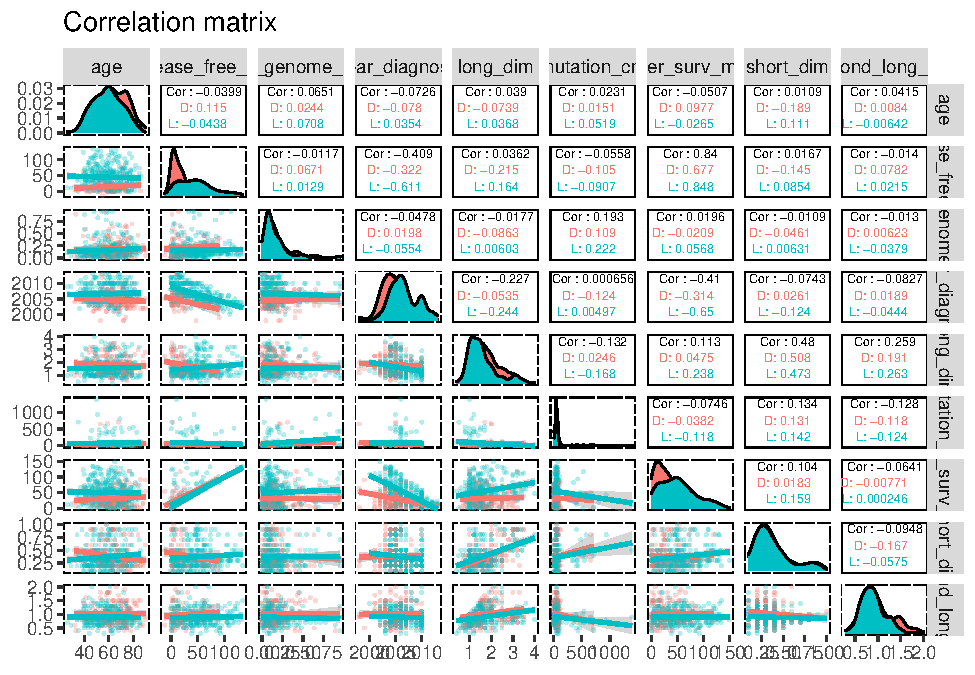
\includegraphics{figs/render-unnamed-chunk-6-1.pdf}

\subsubsection{4.1 Run multiple T-tests on
over\_surv\_stt}\label{run-multiple-t-tests-on-over_surv_stt}

Transform the data into long format

\begin{Shaded}
\begin{Highlighting}[]
\CommentTok{# Put all variables in the same column except `over_surv_stt`, the grouping variable}

\KeywordTok{levels}\NormalTok{(kirc_clinic_numeric}\OperatorTok{$}\NormalTok{over_surv_stt) <-}\StringTok{ }\KeywordTok{c}\NormalTok{(}\StringTok{"DECEASED"}\NormalTok{,}\StringTok{"LIVING"}\NormalTok{)}

\NormalTok{kirc_clinic_numeric.long <-}\StringTok{ }\NormalTok{kirc_clinic_numeric }\OperatorTok
\StringTok{  }\KeywordTok{pivot_longer}\NormalTok{(}\OperatorTok{-}\NormalTok{over_surv_stt, }\DataTypeTok{names_to =} \StringTok{"variables"}\NormalTok{, }\DataTypeTok{values_to =} \StringTok{"value"}\NormalTok{)}

\CommentTok{# Convert to Tidyverse}
\NormalTok{kirc_clinic_numeric.long <-}\StringTok{ }\NormalTok{kirc_clinic_numeric.long[}\OperatorTok{!}\KeywordTok{is.na}\NormalTok{(kirc_clinic_numeric.long}\OperatorTok{$}\NormalTok{value), ]}

\NormalTok{kirc_clinic_numeric.long}\OperatorTok{$}\NormalTok{value.log <-}\StringTok{ }\KeywordTok{log2}\NormalTok{(kirc_clinic_numeric.long}\OperatorTok{$}\NormalTok{value}\OperatorTok{+}\DecValTok{1}\NormalTok{)}
\end{Highlighting}
\end{Shaded}

\begin{verbatim}
## Warning: NaNs produzidos
\end{verbatim}

\begin{Shaded}
\begin{Highlighting}[]
\NormalTok{kirc_clinic_numeric.long }\OperatorTok\StringTok{ }\KeywordTok{sample_n}\NormalTok{(}\DecValTok{6}\NormalTok{)}
\end{Highlighting}
\end{Shaded}

\begin{verbatim}
## # A tibble: 6 x 4
##   over_surv_stt variables        value value.log
##   <fct>         <chr>            <dbl>     <dbl>
## 1 DECEASED      long_dim           1.7     1.43 
## 2 LIVING        year_diagnose   2007      11.0  
## 3 DECEASED      second_long_dim    1.5     1.32 
## 4 DECEASED      year_diagnose   2002      11.0  
## 5 LIVING        short_dim          0.3     0.379
## 6 LIVING        mutation_cnt      17       4.17
\end{verbatim}

Group the data by variables and compare over\_surv\_stt groups

Adjust the p-values and add significance levels

\begin{Shaded}
\begin{Highlighting}[]
\NormalTok{stat.test <-}\StringTok{ }\NormalTok{kirc_clinic_numeric.long }\OperatorTok
\StringTok{  }\KeywordTok{group_by}\NormalTok{(variables) }\OperatorTok
\StringTok{  }\KeywordTok{t_test}\NormalTok{(value }\OperatorTok{~}\StringTok{ }\NormalTok{over_surv_stt) }\OperatorTok
\StringTok{  }\KeywordTok{adjust_pvalue}\NormalTok{(}\DataTypeTok{method =} \StringTok{"BH"}\NormalTok{) }\OperatorTok
\StringTok{  }\KeywordTok{add_significance}\NormalTok{()}
\NormalTok{stat.test}
\end{Highlighting}
\end{Shaded}

\begin{verbatim}
## # A tibble: 9 x 11
##   variables .y.   group1 group2    n1    n2 statistic    df        p    p.adj
##   <chr>     <chr> <chr>  <chr>  <int> <int>     <dbl> <dbl>    <dbl>    <dbl>
## 1 age       value DECEA~ LIVING   177   360     4.89   348. 1.57e- 6 3.53e- 6
## 2 disease_~ value DECEA~ LIVING    78   360   -11.0    188. 5.24e-22 4.72e-21
## 3 frac_gen~ value DECEA~ LIVING   175   353     1.20   344. 2.33e- 1 2.62e- 1
## 4 long_dim  value DECEA~ LIVING   173   329     4.13   363. 4.51e- 5 8.12e- 5
## 5 mutation~ value DECEA~ LIVING   153   298    -1.83   429. 6.79e- 2 8.73e- 2
## 6 over_sur~ value DECEA~ LIVING   177   360    -7.32   451. 1.17e-12 3.51e-12
## 7 second_l~ value DECEA~ LIVING   173   329     4.06   288. 6.23e- 5 9.34e- 5
## 8 short_dim value DECEA~ LIVING   173   329     0.478  345. 6.33e- 1 6.33e- 1
## 9 year_dia~ value DECEA~ LIVING   177   360    -8.90   377. 2.41e-17 1.08e-16
## # ... with 1 more variable: p.adj.signif <chr>
\end{verbatim}

\begin{Shaded}
\begin{Highlighting}[]
\CommentTok{# Create the plot on logscale}
\NormalTok{myplot <-}\StringTok{ }\KeywordTok{ggboxplot}\NormalTok{(}
\NormalTok{  kirc_clinic_numeric.long, }\DataTypeTok{x =} \StringTok{"over_surv_stt"}\NormalTok{, }\DataTypeTok{y =} \StringTok{"value.log"}\NormalTok{,}
  \DataTypeTok{fill =} \StringTok{"over_surv_stt"}\NormalTok{, }\DataTypeTok{palette =} \StringTok{"npg"}\NormalTok{, }\DataTypeTok{legend =} \StringTok{"none"}\NormalTok{, }
  \DataTypeTok{ggtheme =} \KeywordTok{theme_pubr}\NormalTok{(}\DataTypeTok{border =} \OtherTok{TRUE}\NormalTok{)}
\NormalTok{  ) }\OperatorTok{+}
\StringTok{  }\KeywordTok{facet_wrap}\NormalTok{(}\OperatorTok{~}\NormalTok{variables)}
\CommentTok{# Add statistical test p-values}
\NormalTok{stat.test <-}\StringTok{ }\NormalTok{stat.test }\OperatorTok\StringTok{ }\KeywordTok{add_xy_position}\NormalTok{(}\DataTypeTok{x =} \StringTok{"over_surv_stt"}\NormalTok{)}
\NormalTok{myplot }\OperatorTok{+}\StringTok{ }\KeywordTok{stat_pvalue_manual}\NormalTok{(stat.test, }\DataTypeTok{label =} \StringTok{"p.adj.signif"}\NormalTok{)}
\end{Highlighting}
\end{Shaded}

\begin{verbatim}
## Warning: Removed 1 rows containing non-finite values (stat_boxplot).
\end{verbatim}

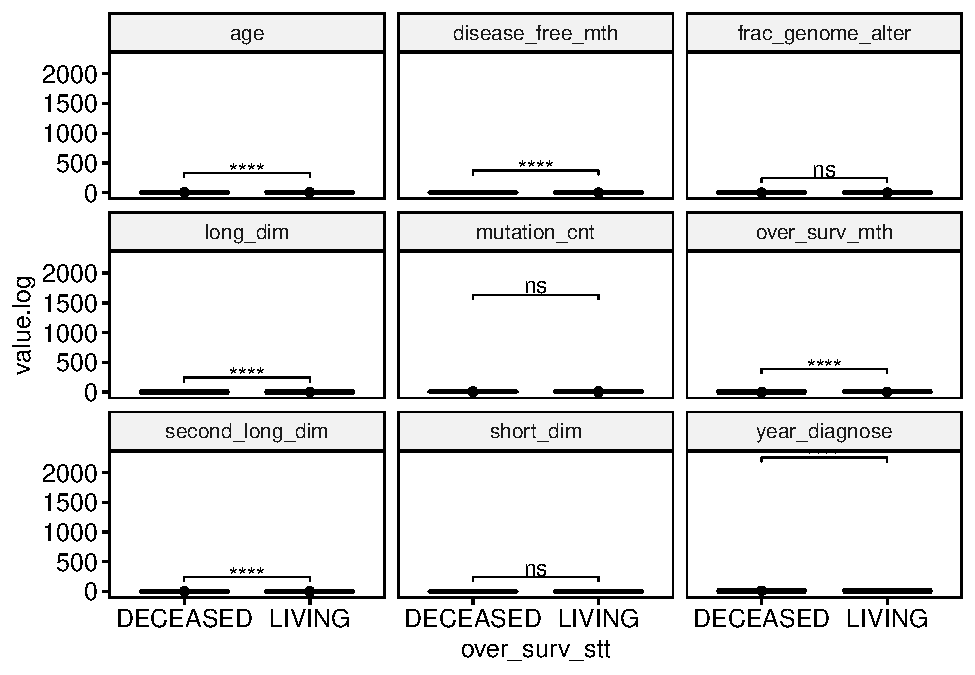
\includegraphics{figs/render-unnamed-chunk-9-1.pdf}

\begin{Shaded}
\begin{Highlighting}[]
\CommentTok{# Group the data by variables and do a graph for each variable}
\NormalTok{graphs <-}\StringTok{ }\NormalTok{kirc_clinic_numeric.long }\OperatorTok
\StringTok{  }\KeywordTok{group_by}\NormalTok{(variables) }\OperatorTok
\StringTok{  }\KeywordTok{doo}\NormalTok{(}
    \OperatorTok{~}\KeywordTok{ggboxplot}\NormalTok{(}
      \DataTypeTok{data =}\NormalTok{., }\DataTypeTok{x =} \StringTok{"over_surv_stt"}\NormalTok{, }\DataTypeTok{y =} \StringTok{"value"}\NormalTok{,}
      \DataTypeTok{fill =} \StringTok{"over_surv_stt"}\NormalTok{, }\DataTypeTok{palette =} \StringTok{"npg"}\NormalTok{, }\DataTypeTok{legend =} \StringTok{"none"}\NormalTok{,}
      \DataTypeTok{ggtheme =} \KeywordTok{theme_pubr}\NormalTok{()}
\NormalTok{      )  }\OperatorTok{+}
\StringTok{      }\KeywordTok{geom_jitter}\NormalTok{(}\DataTypeTok{width =} \FloatTok{0.05}\NormalTok{, }\DataTypeTok{alpha =} \FloatTok{0.2}\NormalTok{, }\DataTypeTok{color =} \StringTok{"orange"}\NormalTok{), }
    \DataTypeTok{result =} \StringTok{"plots"}
\NormalTok{  )}
\NormalTok{graphs}
\end{Highlighting}
\end{Shaded}

\begin{verbatim}
## # A tibble: 9 x 2
##   variables         plots 
##   <chr>             <list>
## 1 age               <gg>  
## 2 disease_free_mth  <gg>  
## 3 frac_genome_alter <gg>  
## 4 long_dim          <gg>  
## 5 mutation_cnt      <gg>  
## 6 over_surv_mth     <gg>  
## 7 second_long_dim   <gg>  
## 8 short_dim         <gg>  
## 9 year_diagnose     <gg>
\end{verbatim}

\begin{Shaded}
\begin{Highlighting}[]
\CommentTok{# Add statitistical tests to each corresponding plot}
\NormalTok{variables <-}\StringTok{ }\NormalTok{graphs}\OperatorTok{$}\NormalTok{variables}
\ControlFlowTok{for}\NormalTok{(i }\ControlFlowTok{in} \DecValTok{1}\OperatorTok{:}\KeywordTok{length}\NormalTok{(variables))\{}
\NormalTok{  graph.i <-}\StringTok{ }\NormalTok{graphs}\OperatorTok{$}\NormalTok{plots[[i]] }\OperatorTok{+}\StringTok{ }
\StringTok{    }\KeywordTok{labs}\NormalTok{(}\DataTypeTok{title =}\NormalTok{ variables[i]) }\OperatorTok{+}
\StringTok{    }\KeywordTok{stat_pvalue_manual}\NormalTok{(stat.test[i, ], }\DataTypeTok{label =} \StringTok{"p.adj.signif"}\NormalTok{)}
  \KeywordTok{print}\NormalTok{(graph.i)}
\NormalTok{\}}
\end{Highlighting}
\end{Shaded}

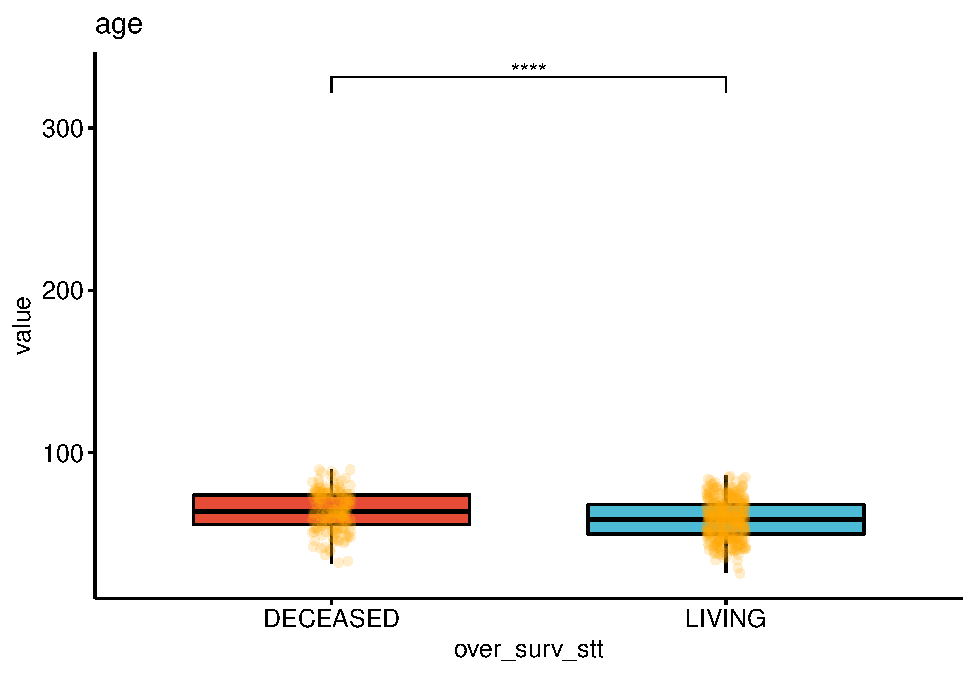
\includegraphics{figs/render-unnamed-chunk-11-1.pdf}
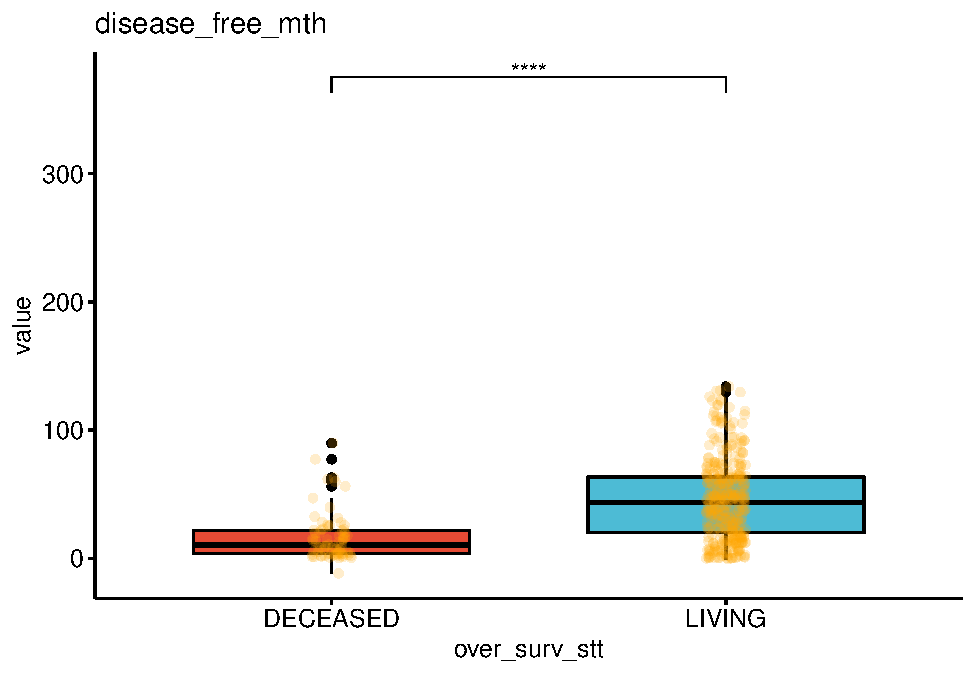
\includegraphics{figs/render-unnamed-chunk-11-2.pdf}
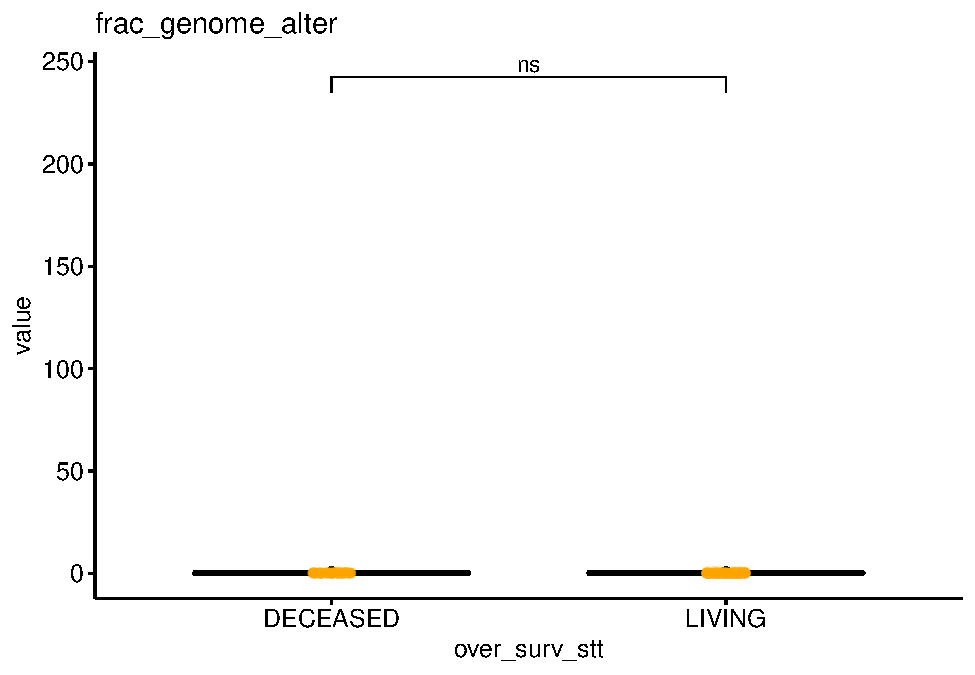
\includegraphics{figs/render-unnamed-chunk-11-3.pdf}
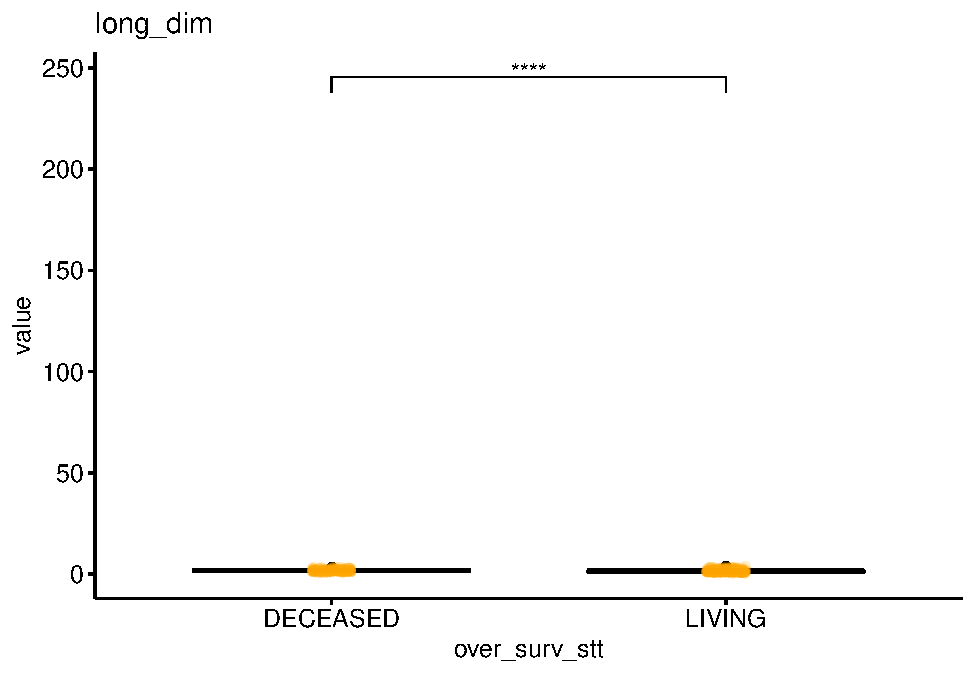
\includegraphics{figs/render-unnamed-chunk-11-4.pdf}
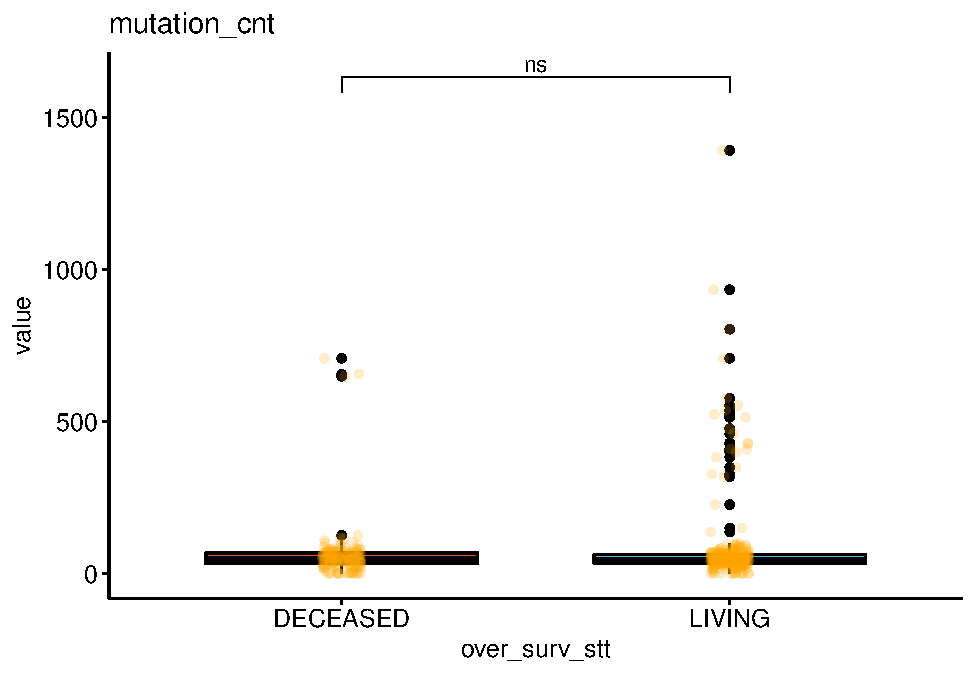
\includegraphics{figs/render-unnamed-chunk-11-5.pdf}
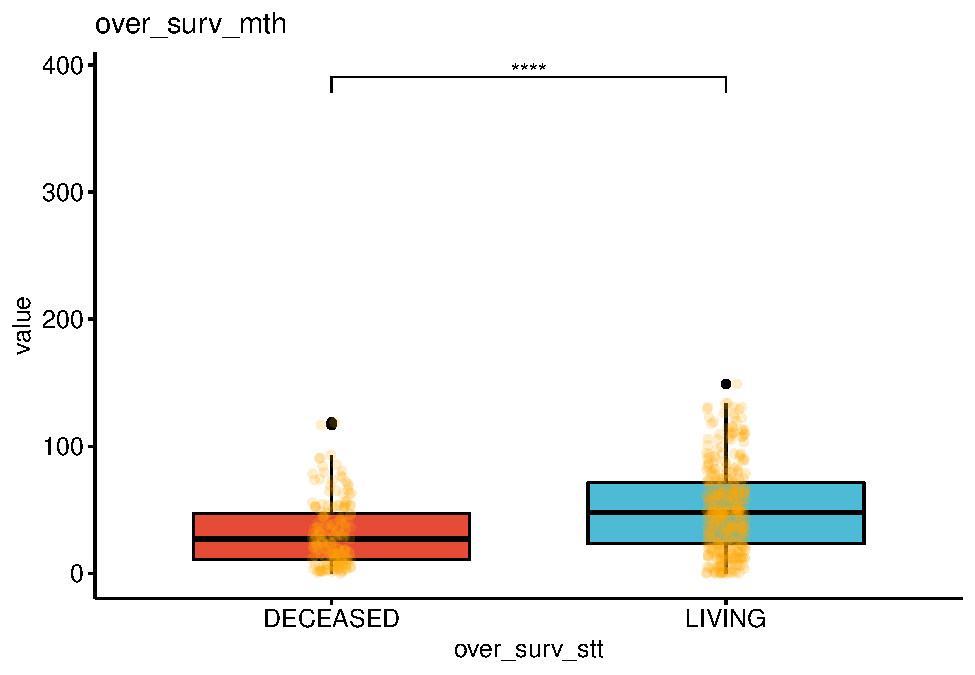
\includegraphics{figs/render-unnamed-chunk-11-6.pdf}
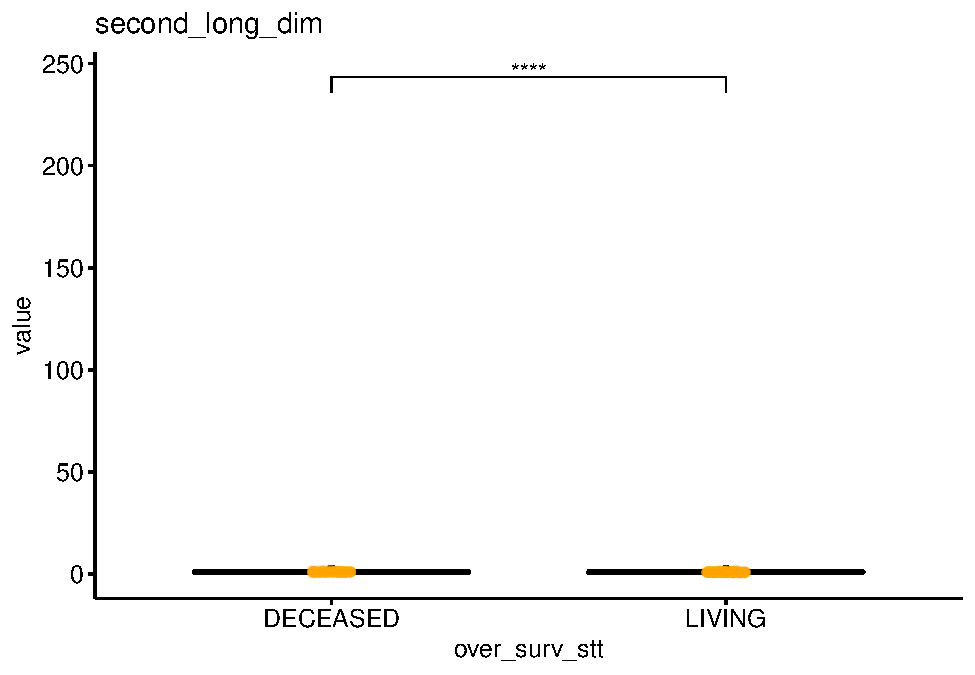
\includegraphics{figs/render-unnamed-chunk-11-7.pdf}
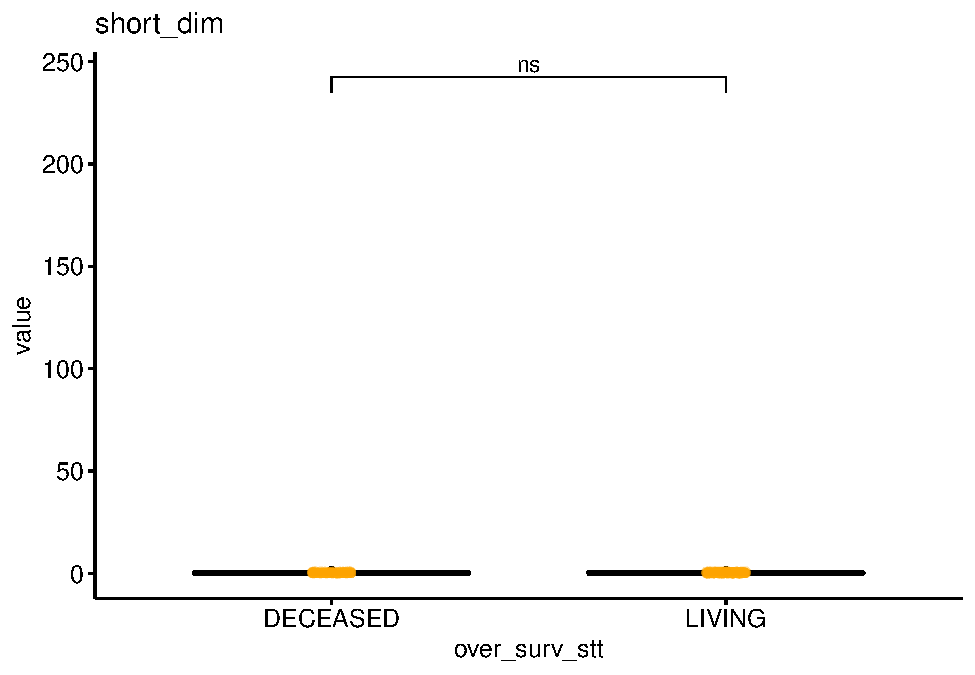
\includegraphics{figs/render-unnamed-chunk-11-8.pdf}
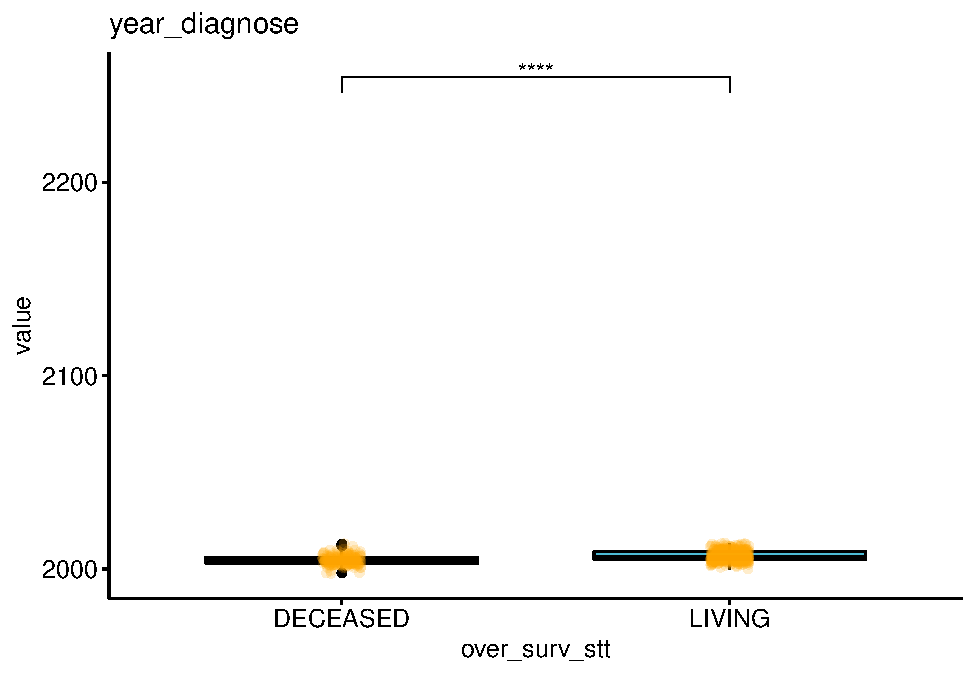
\includegraphics{figs/render-unnamed-chunk-11-9.pdf}

\begin{Shaded}
\begin{Highlighting}[]
\KeywordTok{ggplot}\NormalTok{(kirc_clinic, }\KeywordTok{aes}\NormalTok{(age, }\DataTypeTok{fill=}\NormalTok{ over_surv_stt)) }\OperatorTok{+}
\StringTok{  }\KeywordTok{geom_histogram}\NormalTok{(}\DataTypeTok{bins =} \DecValTok{15}\NormalTok{, }\DataTypeTok{position =} \StringTok{"dodge"}\NormalTok{)}
\end{Highlighting}
\end{Shaded}

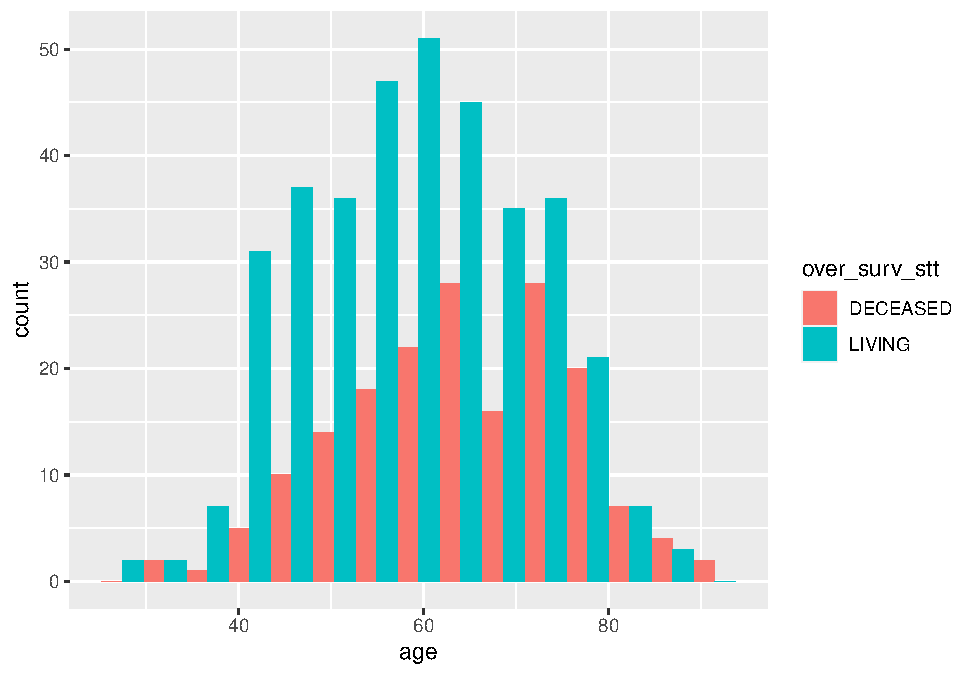
\includegraphics{figs/render-unnamed-chunk-12-1.pdf}

\begin{Shaded}
\begin{Highlighting}[]
\KeywordTok{t.test}\NormalTok{(kirc_clinic}\OperatorTok{$}\NormalTok{age }\OperatorTok{~}\StringTok{ }\NormalTok{kirc_clinic}\OperatorTok{$}\NormalTok{over_surv_stt) }
\end{Highlighting}
\end{Shaded}

\begin{verbatim}
## 
##  Welch Two Sample t-test
## 
## data:  kirc_clinic$age by kirc_clinic$over_surv_stt
## t = 4.887, df = 348.17, p-value = 1.565e-06
## alternative hypothesis: true difference in means is not equal to 0
## 95 percent confidence interval:
##  3.196986 7.503485
## sample estimates:
## mean in group DECEASED   mean in group LIVING 
##               64.18079               58.83056
\end{verbatim}

\begin{Shaded}
\begin{Highlighting}[]
\KeywordTok{ggplot}\NormalTok{(kirc_clinic, }\KeywordTok{aes}\NormalTok{(year_diagnose, }\DataTypeTok{fill=}\NormalTok{ over_surv_stt)) }\OperatorTok{+}
\StringTok{  }\KeywordTok{geom_histogram}\NormalTok{(}\DataTypeTok{bins =} \DecValTok{15}\NormalTok{, }\DataTypeTok{position =} \StringTok{"dodge"}\NormalTok{)}
\end{Highlighting}
\end{Shaded}

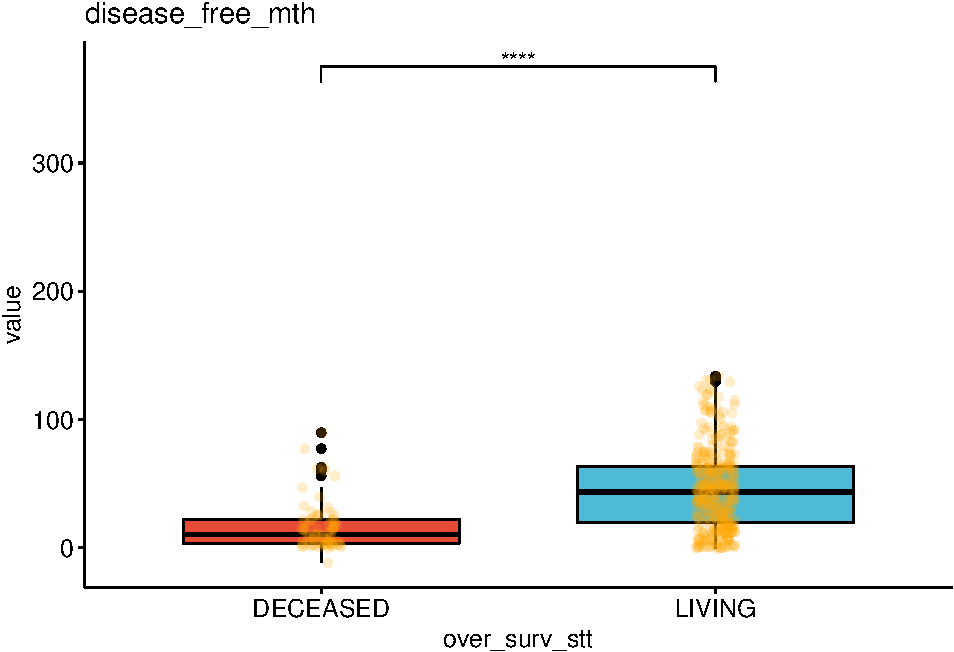
\includegraphics{figs/render-unnamed-chunk-12-2.pdf}

\begin{Shaded}
\begin{Highlighting}[]
\KeywordTok{t.test}\NormalTok{(kirc_clinic}\OperatorTok{$}\NormalTok{year_diagnose }\OperatorTok{~}\StringTok{ }\NormalTok{kirc_clinic}\OperatorTok{$}\NormalTok{over_surv_stt) }
\end{Highlighting}
\end{Shaded}

\begin{verbatim}
## 
##  Welch Two Sample t-test
## 
## data:  kirc_clinic$year_diagnose by kirc_clinic$over_surv_stt
## t = -8.898, df = 377.09, p-value < 2.2e-16
## alternative hypothesis: true difference in means is not equal to 0
## 95 percent confidence interval:
##  -2.510367 -1.601685
## sample estimates:
## mean in group DECEASED   mean in group LIVING 
##               2004.638               2006.694
\end{verbatim}

\begin{Shaded}
\begin{Highlighting}[]
\KeywordTok{ggplot}\NormalTok{(kirc_clinic, }\KeywordTok{aes}\NormalTok{(}\DataTypeTok{x=}\NormalTok{over_surv_stt, }\DataTypeTok{y=}\NormalTok{disease_free_mth)) }\OperatorTok{+}
\StringTok{  }\KeywordTok{geom_boxplot}\NormalTok{(}\DataTypeTok{width =}\NormalTok{ .}\DecValTok{5}\NormalTok{) }\OperatorTok{+}
\StringTok{  }\KeywordTok{geom_jitter}\NormalTok{(}\DataTypeTok{width =} \FloatTok{0.05}\NormalTok{, }\DataTypeTok{alpha =} \FloatTok{0.2}\NormalTok{, }\DataTypeTok{color =} \StringTok{"orange"}\NormalTok{)}
\end{Highlighting}
\end{Shaded}

\begin{verbatim}
## Warning: Removed 99 rows containing non-finite values (stat_boxplot).
\end{verbatim}

\begin{verbatim}
## Warning: Removed 99 rows containing missing values (geom_point).
\end{verbatim}

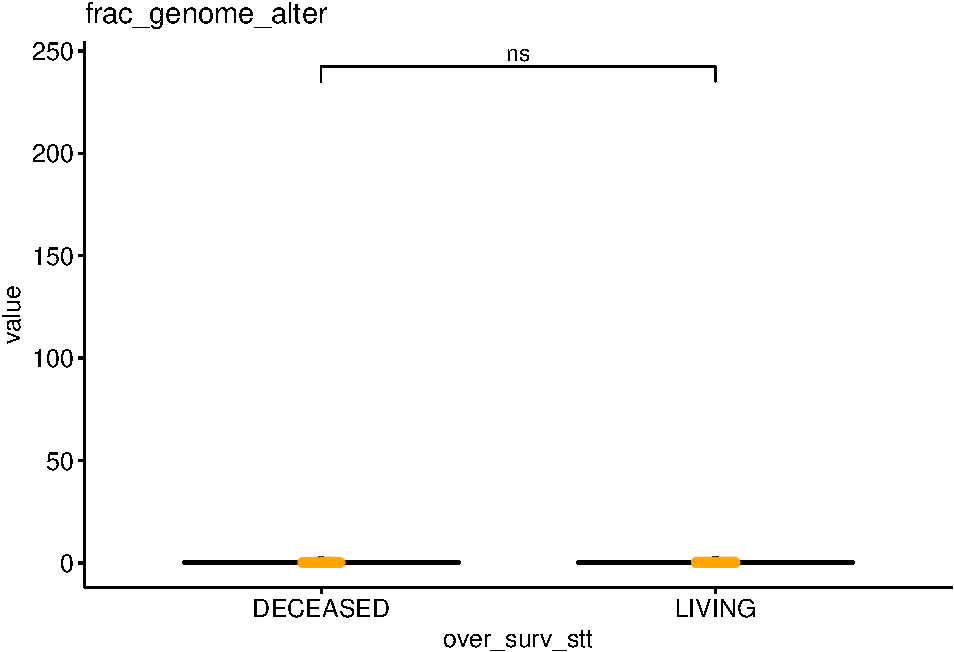
\includegraphics{figs/render-unnamed-chunk-12-3.pdf}

\begin{Shaded}
\begin{Highlighting}[]
\KeywordTok{t.test}\NormalTok{(kirc_clinic}\OperatorTok{$}\NormalTok{disease_free_mth }\OperatorTok{~}\StringTok{ }\NormalTok{kirc_clinic}\OperatorTok{$}\NormalTok{over_surv_stt) }
\end{Highlighting}
\end{Shaded}

\begin{verbatim}
## 
##  Welch Two Sample t-test
## 
## data:  kirc_clinic$disease_free_mth by kirc_clinic$over_surv_stt
## t = -10.985, df = 188.22, p-value < 2.2e-16
## alternative hypothesis: true difference in means is not equal to 0
## 95 percent confidence interval:
##  -34.63580 -24.08972
## sample estimates:
## mean in group DECEASED   mean in group LIVING 
##               16.10846               45.47122
\end{verbatim}

\begin{Shaded}
\begin{Highlighting}[]
\KeywordTok{ggplot}\NormalTok{(kirc_clinic, }\KeywordTok{aes}\NormalTok{(}\DataTypeTok{x=}\NormalTok{over_surv_stt, }\DataTypeTok{y=}\NormalTok{frac_genome_alter)) }\OperatorTok{+}
\StringTok{  }\KeywordTok{geom_boxplot}\NormalTok{(}\DataTypeTok{width =}\NormalTok{ .}\DecValTok{5}\NormalTok{) }\OperatorTok{+}
\StringTok{  }\KeywordTok{geom_jitter}\NormalTok{(}\DataTypeTok{width =} \FloatTok{0.05}\NormalTok{, }\DataTypeTok{alpha =} \FloatTok{0.2}\NormalTok{, }\DataTypeTok{color =} \StringTok{"orange"}\NormalTok{)}
\end{Highlighting}
\end{Shaded}

\begin{verbatim}
## Warning: Removed 9 rows containing non-finite values (stat_boxplot).
\end{verbatim}

\begin{verbatim}
## Warning: Removed 9 rows containing missing values (geom_point).
\end{verbatim}

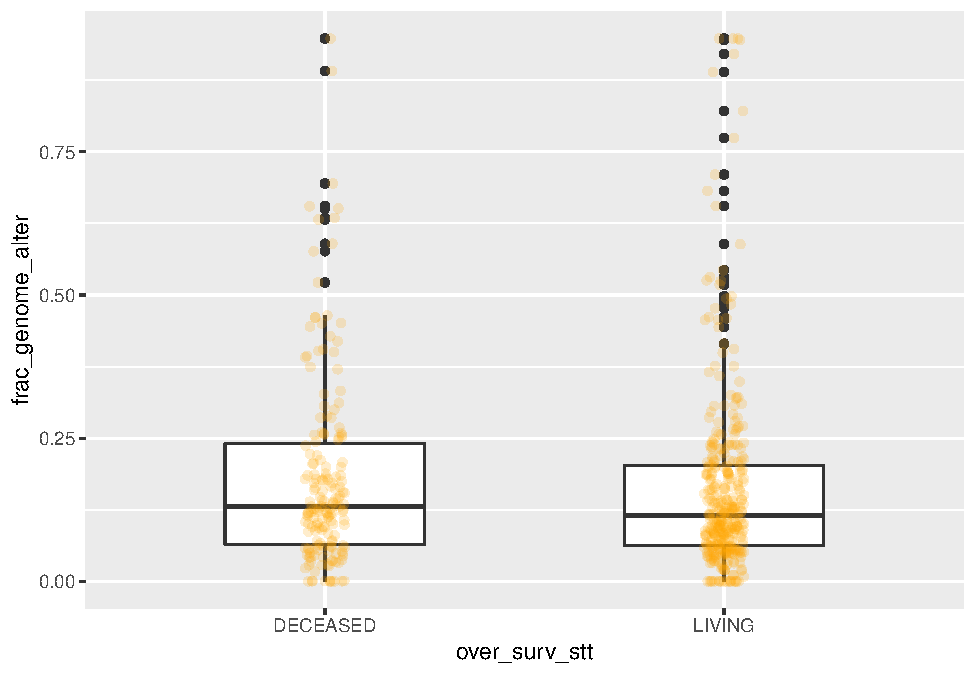
\includegraphics{figs/render-unnamed-chunk-12-4.pdf}

\begin{Shaded}
\begin{Highlighting}[]
\KeywordTok{t.test}\NormalTok{(kirc_clinic}\OperatorTok{$}\NormalTok{frac_genome_alter }\OperatorTok{~}\StringTok{ }\NormalTok{kirc_clinic}\OperatorTok{$}\NormalTok{over_surv_stt)}
\end{Highlighting}
\end{Shaded}

\begin{verbatim}
## 
##  Welch Two Sample t-test
## 
## data:  kirc_clinic$frac_genome_alter by kirc_clinic$over_surv_stt
## t = 1.196, df = 343.6, p-value = 0.2325
## alternative hypothesis: true difference in means is not equal to 0
## 95 percent confidence interval:
##  -0.01199882  0.04923234
## sample estimates:
## mean in group DECEASED   mean in group LIVING 
##              0.1826051              0.1639884
\end{verbatim}

\begin{Shaded}
\begin{Highlighting}[]
\KeywordTok{ggplot}\NormalTok{(kirc_clinic, }\KeywordTok{aes}\NormalTok{(}\DataTypeTok{x=}\NormalTok{over_surv_stt, }\DataTypeTok{y=}\NormalTok{long_dim)) }\OperatorTok{+}
\StringTok{  }\KeywordTok{geom_boxplot}\NormalTok{(}\DataTypeTok{width =}\NormalTok{ .}\DecValTok{5}\NormalTok{) }\OperatorTok{+}
\StringTok{  }\KeywordTok{geom_jitter}\NormalTok{(}\DataTypeTok{width =} \FloatTok{0.05}\NormalTok{, }\DataTypeTok{alpha =} \FloatTok{0.2}\NormalTok{, }\DataTypeTok{color =} \StringTok{"orange"}\NormalTok{)}
\end{Highlighting}
\end{Shaded}

\begin{verbatim}
## Warning: Removed 35 rows containing non-finite values (stat_boxplot).
\end{verbatim}

\begin{verbatim}
## Warning: Removed 35 rows containing missing values (geom_point).
\end{verbatim}

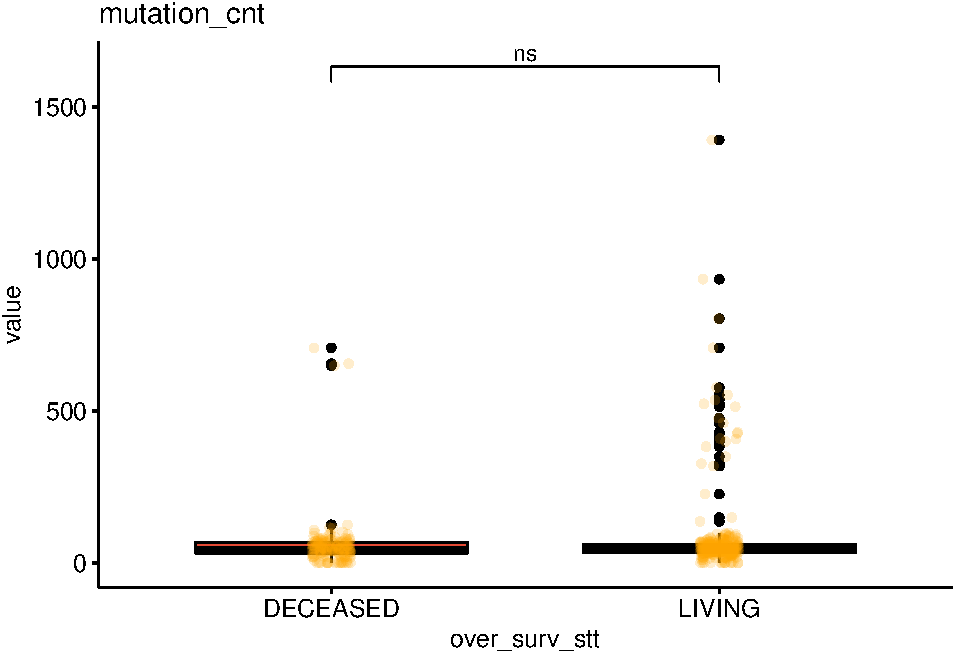
\includegraphics{figs/render-unnamed-chunk-12-5.pdf}

\begin{Shaded}
\begin{Highlighting}[]
\KeywordTok{t.test}\NormalTok{(kirc_clinic}\OperatorTok{$}\NormalTok{long_dim }\OperatorTok{~}\StringTok{ }\NormalTok{kirc_clinic}\OperatorTok{$}\NormalTok{over_surv_stt)}
\end{Highlighting}
\end{Shaded}

\begin{verbatim}
## 
##  Welch Two Sample t-test
## 
## data:  kirc_clinic$long_dim by kirc_clinic$over_surv_stt
## t = 4.1297, df = 363.45, p-value = 4.51e-05
## alternative hypothesis: true difference in means is not equal to 0
## 95 percent confidence interval:
##  0.1295804 0.3651751
## sample estimates:
## mean in group DECEASED   mean in group LIVING 
##               1.824277               1.576900
\end{verbatim}

\begin{Shaded}
\begin{Highlighting}[]
\KeywordTok{ggplot}\NormalTok{(kirc_clinic, }\KeywordTok{aes}\NormalTok{(}\DataTypeTok{x=}\NormalTok{over_surv_stt, }\DataTypeTok{y=}\NormalTok{mutation_cnt)) }\OperatorTok{+}
\StringTok{  }\KeywordTok{geom_boxplot}\NormalTok{(}\DataTypeTok{width =}\NormalTok{ .}\DecValTok{5}\NormalTok{) }\OperatorTok{+}
\StringTok{  }\KeywordTok{geom_jitter}\NormalTok{(}\DataTypeTok{width =} \FloatTok{0.05}\NormalTok{, }\DataTypeTok{alpha =} \FloatTok{0.2}\NormalTok{, }\DataTypeTok{color =} \StringTok{"orange"}\NormalTok{)}
\end{Highlighting}
\end{Shaded}

\begin{verbatim}
## Warning: Removed 86 rows containing non-finite values (stat_boxplot).
\end{verbatim}

\begin{verbatim}
## Warning: Removed 86 rows containing missing values (geom_point).
\end{verbatim}

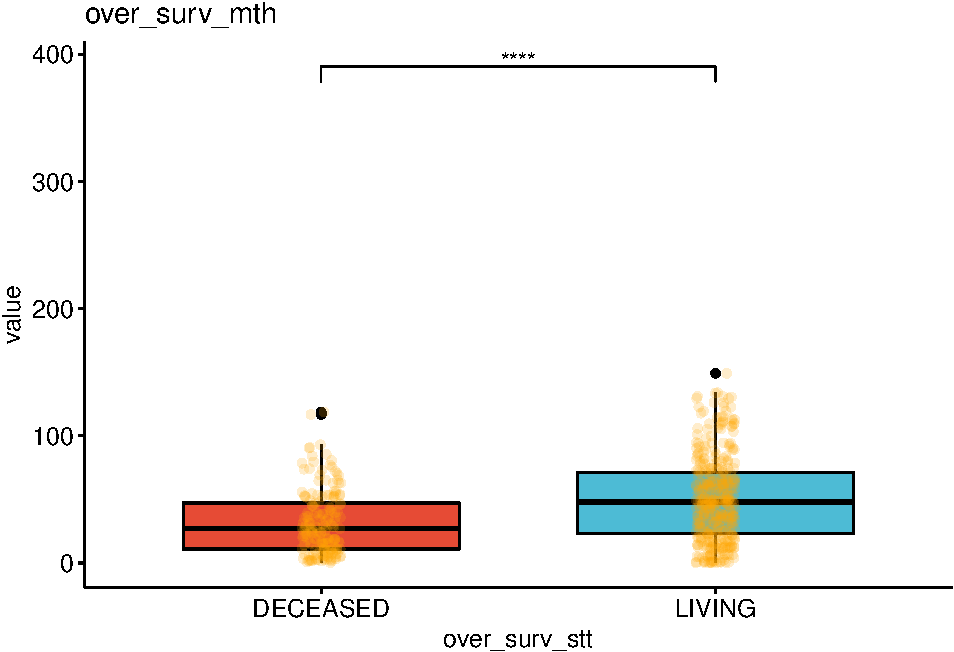
\includegraphics{figs/render-unnamed-chunk-12-6.pdf}

\begin{Shaded}
\begin{Highlighting}[]
\KeywordTok{t.test}\NormalTok{(kirc_clinic}\OperatorTok{$}\NormalTok{mutation_cnt }\OperatorTok{~}\StringTok{ }\NormalTok{kirc_clinic}\OperatorTok{$}\NormalTok{over_surv_stt)}
\end{Highlighting}
\end{Shaded}

\begin{verbatim}
## 
##  Welch Two Sample t-test
## 
## data:  kirc_clinic$mutation_cnt by kirc_clinic$over_surv_stt
## t = -1.8306, df = 428.83, p-value = 0.06786
## alternative hypothesis: true difference in means is not equal to 0
## 95 percent confidence interval:
##  -41.980661   1.492307
## sample estimates:
## mean in group DECEASED   mean in group LIVING 
##               60.47059               80.71477
\end{verbatim}

\begin{Shaded}
\begin{Highlighting}[]
\KeywordTok{ggplot}\NormalTok{(kirc_clinic, }\KeywordTok{aes}\NormalTok{(}\DataTypeTok{x=}\NormalTok{over_surv_stt, }\DataTypeTok{y=}\NormalTok{over_surv_mth)) }\OperatorTok{+}
\StringTok{  }\KeywordTok{geom_boxplot}\NormalTok{(}\DataTypeTok{width =}\NormalTok{ .}\DecValTok{5}\NormalTok{) }\OperatorTok{+}
\StringTok{  }\KeywordTok{geom_jitter}\NormalTok{(}\DataTypeTok{width =} \FloatTok{0.05}\NormalTok{, }\DataTypeTok{alpha =} \FloatTok{0.2}\NormalTok{, }\DataTypeTok{color =} \StringTok{"orange"}\NormalTok{)}
\end{Highlighting}
\end{Shaded}

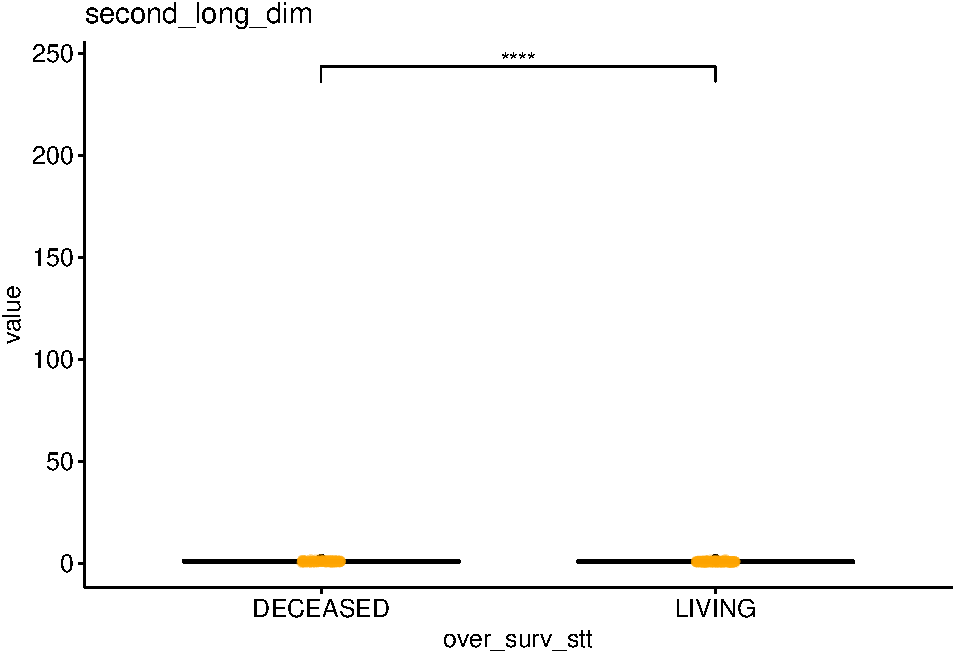
\includegraphics{figs/render-unnamed-chunk-12-7.pdf}

\begin{Shaded}
\begin{Highlighting}[]
\KeywordTok{t.test}\NormalTok{(kirc_clinic}\OperatorTok{$}\NormalTok{over_surv_mth }\OperatorTok{~}\StringTok{ }\NormalTok{kirc_clinic}\OperatorTok{$}\NormalTok{over_surv_stt)}
\end{Highlighting}
\end{Shaded}

\begin{verbatim}
## 
##  Welch Two Sample t-test
## 
## data:  kirc_clinic$over_surv_mth by kirc_clinic$over_surv_stt
## t = -7.3172, df = 450.92, p-value = 1.169e-12
## alternative hypothesis: true difference in means is not equal to 0
## 95 percent confidence interval:
##  -23.99320 -13.83372
## sample estimates:
## mean in group DECEASED   mean in group LIVING 
##               31.57734               50.49081
\end{verbatim}

\begin{Shaded}
\begin{Highlighting}[]
\KeywordTok{ggplot}\NormalTok{(kirc_clinic, }\KeywordTok{aes}\NormalTok{(}\DataTypeTok{x=}\NormalTok{over_surv_stt, }\DataTypeTok{y=}\NormalTok{short_dim)) }\OperatorTok{+}
\StringTok{  }\KeywordTok{geom_boxplot}\NormalTok{(}\DataTypeTok{width =}\NormalTok{ .}\DecValTok{5}\NormalTok{) }\OperatorTok{+}
\StringTok{  }\KeywordTok{geom_jitter}\NormalTok{(}\DataTypeTok{width =} \FloatTok{0.05}\NormalTok{, }\DataTypeTok{alpha =} \FloatTok{0.2}\NormalTok{, }\DataTypeTok{color =} \StringTok{"orange"}\NormalTok{)}
\end{Highlighting}
\end{Shaded}

\begin{verbatim}
## Warning: Removed 35 rows containing non-finite values (stat_boxplot).
\end{verbatim}

\begin{verbatim}
## Warning: Removed 35 rows containing missing values (geom_point).
\end{verbatim}

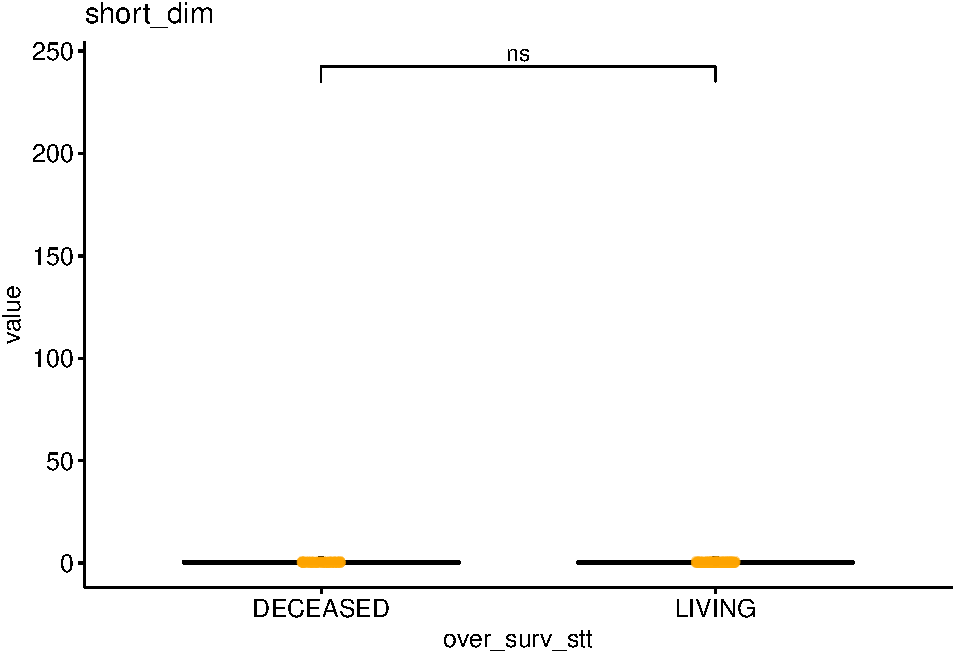
\includegraphics{figs/render-unnamed-chunk-12-8.pdf}

\begin{Shaded}
\begin{Highlighting}[]
\KeywordTok{t.test}\NormalTok{(kirc_clinic}\OperatorTok{$}\NormalTok{short_dim }\OperatorTok{~}\StringTok{ }\NormalTok{kirc_clinic}\OperatorTok{$}\NormalTok{over_surv_stt)}
\end{Highlighting}
\end{Shaded}

\begin{verbatim}
## 
##  Welch Two Sample t-test
## 
## data:  kirc_clinic$short_dim by kirc_clinic$over_surv_stt
## t = 0.47841, df = 344.68, p-value = 0.6327
## alternative hypothesis: true difference in means is not equal to 0
## 95 percent confidence interval:
##  -0.02935985  0.04823295
## sample estimates:
## mean in group DECEASED   mean in group LIVING 
##              0.3820809              0.3726444
\end{verbatim}

\begin{Shaded}
\begin{Highlighting}[]
\KeywordTok{ggplot}\NormalTok{(kirc_clinic, }\KeywordTok{aes}\NormalTok{(}\DataTypeTok{x=}\NormalTok{over_surv_stt, }\DataTypeTok{y=}\NormalTok{second_long_dim)) }\OperatorTok{+}
\StringTok{  }\KeywordTok{geom_boxplot}\NormalTok{(}\DataTypeTok{width =}\NormalTok{ .}\DecValTok{5}\NormalTok{) }\OperatorTok{+}
\StringTok{  }\KeywordTok{geom_jitter}\NormalTok{(}\DataTypeTok{width =} \FloatTok{0.05}\NormalTok{, }\DataTypeTok{alpha =} \FloatTok{0.2}\NormalTok{, }\DataTypeTok{color =} \StringTok{"orange"}\NormalTok{)}
\end{Highlighting}
\end{Shaded}

\begin{verbatim}
## Warning: Removed 35 rows containing non-finite values (stat_boxplot).

## Warning: Removed 35 rows containing missing values (geom_point).
\end{verbatim}

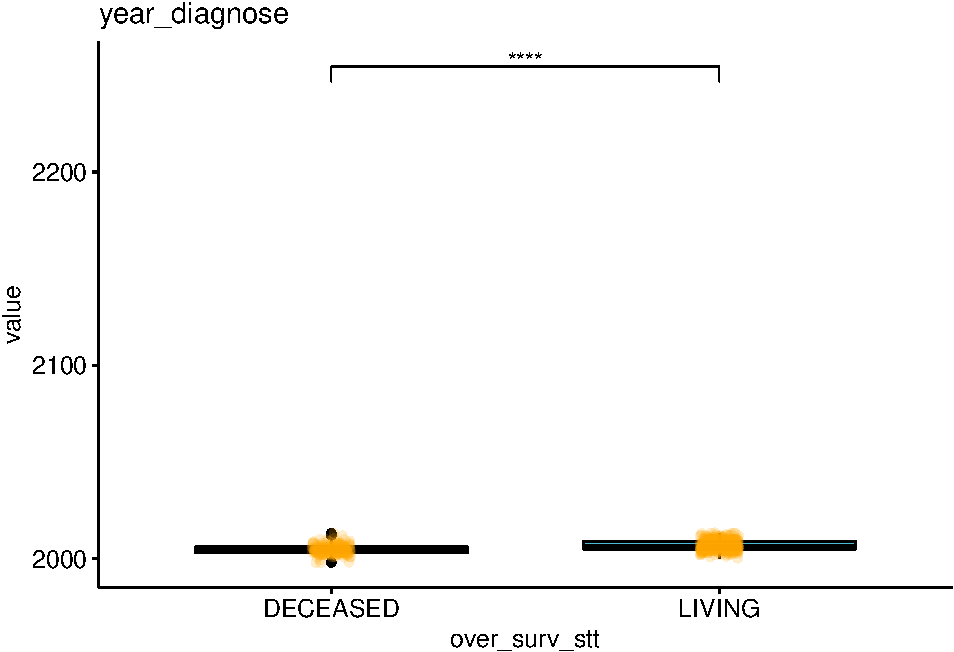
\includegraphics{figs/render-unnamed-chunk-12-9.pdf}

\begin{Shaded}
\begin{Highlighting}[]
\KeywordTok{t.test}\NormalTok{(kirc_clinic}\OperatorTok{$}\NormalTok{second_long_dim }\OperatorTok{~}\StringTok{ }\NormalTok{kirc_clinic}\OperatorTok{$}\NormalTok{over_surv_stt)}
\end{Highlighting}
\end{Shaded}

\begin{verbatim}
## 
##  Welch Two Sample t-test
## 
## data:  kirc_clinic$second_long_dim by kirc_clinic$over_surv_stt
## t = 4.0639, df = 287.92, p-value = 6.231e-05
## alternative hypothesis: true difference in means is not equal to 0
## 95 percent confidence interval:
##  0.06333111 0.18229322
## sample estimates:
## mean in group DECEASED   mean in group LIVING 
##              1.0173410              0.8945289
\end{verbatim}

\subsection{5. Categorical variables
vs.~over\_surv\_stt}\label{categorical-variables-vs.over_surv_stt}

\subsection{5.1 Checking categorical
variables}\label{checking-categorical-variables}

\begin{verbatim}
##  metastasis_stg neoplasm_ln_stg    neoplasm_stg tumor_stg
##  M0  :426       N0:240          Stage I  :269   T1:275   
##  M1  : 79       N1: 17          Stage II : 57   T2: 69   
##  MX  : 30       NX:280          Stage III:125   T3:182   
##  NA's:  2                       Stage IV : 83   T4: 11   
##                                 NA's     :  3            
##                                                          
##             disease_free_stt                  ethnicity   histology_grd
##  DiseaseFree        :311     HISPANIC OR LATINO    : 26   G1  : 14     
##  Recurred/Progressed:127     NOT HISPANIC OR LATINO:359   G2  :230     
##  NA's               : 99     NA's                  :152   G3  :207     
##                                                           G4  : 78     
##                                                           GX  :  5     
##                                                           NA's:  3     
##     hemoglobin  neoadj_therapy prior_cancer   tumor_lateral primer_ln_ind3
##  Elevated:  5   No :519        No :459      Bilateral:  1   NO  :395      
##  Low     :263   Yes: 18        Yes: 78      Left     :253   YES :135      
##  Normal  :186                               Right    :283   NA's:  7      
##  NA's    : 83                                                             
##                                                                           
##                                                                           
##   over_surv_stt     platelet   tissue_prospect                        race    
##  DECEASED:177   Elevated: 38   NO  :465        BLACK OR AFRICAN AMERICAN: 56  
##  LIVING  :360   Low     : 46   YES : 52        WHITE                    :466  
##                 Normal  :360   NA's: 20        NA's                     : 15  
##                 NA's    : 93                                                  
##                                                                               
##                                                                               
##  tissue_retrospect     serum_ca      gender    tissue_site  person_neoplasm_stt
##  NO  : 53          Elevated: 10   Female:191   A     : 79   TUMOR FREE:361     
##  YES :466          Low     :204   Male  :346   B     :303   WITH TUMOR:141     
##  NA's: 18          Normal  :151                C     :127   NA's      : 35     
##                    NA's    :172                OTHERS: 28                      
##                                                                                
##                                                                                
##        wbc     
##  Elevated:164  
##  Low     :  9  
##  Normal  :268  
##  NA's    : 96  
##                
## 
\end{verbatim}

Tabulation and chi-square test

\begin{Shaded}
\begin{Highlighting}[]
\CommentTok{# # talvez isso possa sair uma vez que ja tem a mesma analise com tablefit}
\CommentTok{# }
\CommentTok{# t_metas_stg <- table(kirc_clinic$metastasis_stg, kirc_clinic$over_surv_stt, exclude = NULL)}
\CommentTok{# t_metas_stg <- addmargins(round(100*prop.table(t_metas_stg)))}
\CommentTok{# t_metas_stg}
\CommentTok{# chisq.test(x = kirc_clinic$metastasis_stg, y = kirc_clinic$over_surv_stt) }
\CommentTok{# }
\CommentTok{# t_lynph <- table(kirc_clinic$neoplasm_ln_stg, kirc_clinic$over_surv_stt, exclude = NULL)}
\CommentTok{# t_lynph <- addmargins(round(100*prop.table(t_lynph)))}
\CommentTok{# t_lynph}
\CommentTok{# chisq.test(x = kirc_clinic$neoplasm_ln_stg, y = kirc_clinic$over_surv_stt) }
\CommentTok{# }
\CommentTok{# t_neop <- table(kirc_clinic$neoplasm_stg, kirc_clinic$over_surv_stt, exclude = NULL)}
\CommentTok{# t_neop <- addmargins(round(100*prop.table(t_neop)))}
\CommentTok{# t_neop}
\CommentTok{# chisq.test(x = kirc_clinic$neoplasm_stg, y = kirc_clinic$over_surv_stt) }
\CommentTok{# }
\CommentTok{# t_tumor <- table(kirc_clinic$tumor_stg, kirc_clinic$over_surv_stt, exclude = NULL)}
\CommentTok{# t_tumor <- addmargins(round(100*prop.table(t_tumor)))}
\CommentTok{# t_tumor}
\CommentTok{# chisq.test(x = kirc_clinic$tumor_stg, y = kirc_clinic$over_surv_stt) }
\CommentTok{# }
\CommentTok{# t_free <- table(kirc_clinic$disease_free_stt, kirc_clinic$over_surv_stt, exclude = NULL)}
\CommentTok{# t_free <- addmargins(round(100*prop.table(t_free)))}
\CommentTok{# t_free}
\CommentTok{# chisq.test(x = kirc_clinic$disease_free_stt, y = kirc_clinic$over_surv_stt) }
\CommentTok{# }
\CommentTok{# t_prior <- table(kirc_clinic$prior_cancer, kirc_clinic$over_surv_stt, exclude = NULL)}
\CommentTok{# t_prior <- addmargins(round(100*prop.table(t_prior)))}
\CommentTok{# t_prior}
\CommentTok{# chisq.test(x = kirc_clinic$prior_cancer, y = kirc_clinic$over_surv_stt) }
\CommentTok{# }
\CommentTok{# t_neo <- table(kirc_clinic$neoadj_therapy, kirc_clinic$over_surv_stt, exclude = NULL)}
\CommentTok{# t_neo <- addmargins(round(100*prop.table(t_neo)))}
\CommentTok{# t_neo}
\CommentTok{# chisq.test(x = kirc_clinic$neoadj_therapy, y = kirc_clinic$over_surv_stt) }
\CommentTok{# }
\CommentTok{# t_platelet <- table(kirc_clinic$platelet, kirc_clinic$over_surv_stt, exclude = NULL)}
\CommentTok{# t_platelet <- addmargins(round(100*prop.table(t_platelet)))}
\CommentTok{# t_platelet}
\CommentTok{# chisq.test(x = kirc_clinic$platelet, y = kirc_clinic$over_surv_stt)}
\CommentTok{# }
\CommentTok{# t_prospect <- table(kirc_clinic$tissue_prospect, kirc_clinic$over_surv_stt, exclude = NULL)}
\CommentTok{# t_prospect <- addmargins(round(100*prop.table(t_prospect)))}
\CommentTok{# t_prospect}
\CommentTok{# chisq.test(x = kirc_clinic$tissue_prospect, y = kirc_clinic$over_surv_stt)}
\CommentTok{# }
\CommentTok{# t_race <- table(kirc_clinic$race, kirc_clinic$over_surv_stt, exclude = NULL)}
\CommentTok{# t_race <- addmargins(round(100*prop.table(t_race)))}
\CommentTok{# t_race}
\CommentTok{# chisq.test(x = kirc_clinic$race, y = kirc_clinic$over_surv_stt) }
\CommentTok{# }
\CommentTok{# t_retros <- table(kirc_clinic$tissue_retrospect, kirc_clinic$over_surv_stt, exclude = NULL)}
\CommentTok{# t_retros <- addmargins(round(100*prop.table(t_retros)))}
\CommentTok{# t_retros}
\CommentTok{# chisq.test(x = kirc_clinic$tissue_retrospect, y = kirc_clinic$over_surv_stt)}
\CommentTok{# }
\CommentTok{# t_ca <- table(kirc_clinic$serum_ca, kirc_clinic$over_surv_stt, exclude = NULL)}
\CommentTok{# t_ca <- addmargins(round(100*prop.table(t_ca)))}
\CommentTok{# t_ca}
\CommentTok{# chisq.test(x = kirc_clinic$serum_ca, y = kirc_clinic$over_surv_stt) }
\CommentTok{# }
\CommentTok{# t_gender <- table(kirc_clinic$gender, kirc_clinic$over_surv_stt, exclude = NULL)}
\CommentTok{# t_gender <- addmargins(round(100*prop.table(t_gender)))}
\CommentTok{# t_gender}
\CommentTok{# chisq.test(x = kirc_clinic$gender, y = kirc_clinic$over_surv_stt) }
\CommentTok{# }
\CommentTok{# t_site <- table(kirc_clinic$tissue_site, kirc_clinic$over_surv_stt, exclude = NULL)}
\CommentTok{# t_site <- addmargins(round(100*prop.table(t_site)))}
\CommentTok{# t_site}
\CommentTok{# chisq.test(x = kirc_clinic$tissue_site, y = kirc_clinic$over_surv_stt) }
\CommentTok{# }
\CommentTok{# t_neop_st <- table(kirc_clinic$person_neoplasm_stt, kirc_clinic$over_surv_stt, exclude = NULL)}
\CommentTok{# t_neop_st <- addmargins(round(100*prop.table(t_neop_st)))}
\CommentTok{# t_neop_st}
\CommentTok{# chisq.test(x = kirc_clinic$person_neoplasm_stt, y = kirc_clinic$over_surv_stt) }
\CommentTok{# }
\CommentTok{# t_wbc <- table(kirc_clinic$wbc, kirc_clinic$over_surv_stt, exclude = NULL)}
\CommentTok{# t_wbc <- addmargins(round(100*prop.table(t_wbc)))}
\CommentTok{# t_wbc}
\CommentTok{# chisq.test(x = kirc_clinic$wbc, y = kirc_clinic$over_surv_stt) }
\end{Highlighting}
\end{Shaded}

\subsection{7. FinalFit}\label{finalfit}

Summarise variables/factors by a categorical variable

\begin{Shaded}
\begin{Highlighting}[]
\CommentTok{#  warning=FALSE}
\NormalTok{explanatory_char <-}\StringTok{ }\KeywordTok{names}\NormalTok{(kirc_clinic }\OperatorTok
\StringTok{              }\KeywordTok{select}\NormalTok{(}\OperatorTok{-}\NormalTok{over_surv_stt) }\OperatorTok
\StringTok{              }\KeywordTok{select_if}\NormalTok{(is.factor))}
\NormalTok{dependent <-}\StringTok{  'over_surv_stt'}

\NormalTok{table_fit <-}\StringTok{ }\NormalTok{kirc_clinic }\OperatorTok
\StringTok{  }\KeywordTok{summary_factorlist}\NormalTok{(dependent, explanatory_char, }\DataTypeTok{p=}\OtherTok{TRUE}\NormalTok{, }\DataTypeTok{add_dependent_label=}\OtherTok{TRUE}\NormalTok{,  }\DataTypeTok{na_include =} \OtherTok{TRUE}\NormalTok{)}
\end{Highlighting}
\end{Shaded}

\begin{verbatim}
## Warning in chisq.test(tumor_stg, over_surv_stt): Chi-squared approximation may
## be incorrect
\end{verbatim}

\begin{verbatim}
## Warning in chisq.test(histology_grd, over_surv_stt): Chi-squared approximation
## may be incorrect
\end{verbatim}

\begin{verbatim}
## Warning in chisq.test(hemoglobin, over_surv_stt): Chi-squared approximation may
## be incorrect
\end{verbatim}

\begin{verbatim}
## Warning in chisq.test(tumor_lateral, over_surv_stt): Chi-squared approximation
## may be incorrect
\end{verbatim}

\begin{verbatim}
## Warning in chisq.test(serum_ca, over_surv_stt): Chi-squared approximation may be
## incorrect
\end{verbatim}

\begin{verbatim}
## Warning in chisq.test(wbc, over_surv_stt): Chi-squared approximation may be
## incorrect
\end{verbatim}

\begin{Shaded}
\begin{Highlighting}[]
\NormalTok{knitr}\OperatorTok{::}\KeywordTok{kable}\NormalTok{(table_fit, }\DataTypeTok{row.names=}\OtherTok{FALSE}\NormalTok{, }\DataTypeTok{align=}\KeywordTok{c}\NormalTok{(}\StringTok{"l"}\NormalTok{, }\StringTok{"l"}\NormalTok{, }\StringTok{"r"}\NormalTok{, }\StringTok{"r"}\NormalTok{, }\StringTok{"r"}\NormalTok{))}
\end{Highlighting}
\end{Shaded}

\begin{longtable}[]{@{}llrrr@{}}
\toprule
Dependent: over\_surv\_stt & & DECEASED & LIVING & p\tabularnewline
\midrule
\endhead
metastasis\_stg & M0 & 110 (62.1) & 316 (87.8) &
\textless{}0.001\tabularnewline
& M1 & 64 (36.2) & 15 (4.2) &\tabularnewline
& MX & 3 (1.7) & 27 (7.5) &\tabularnewline
& (Missing) & & 2 (0.6) &\tabularnewline
neoplasm\_ln\_stg & N0 & 85 (48.0) & 155 (43.1) & 0.001\tabularnewline
& N1 & 12 (6.8) & 5 (1.4) &\tabularnewline
& NX & 80 (45.2) & 200 (55.6) &\tabularnewline
neoplasm\_stg & Stage I & 45 (25.4) & 224 (62.2) &
\textless{}0.001\tabularnewline
& Stage II & 13 (7.3) & 44 (12.2) &\tabularnewline
& Stage III & 51 (28.8) & 74 (20.6) &\tabularnewline
& Stage IV & 67 (37.9) & 16 (4.4) &\tabularnewline
& (Missing) & 1 (0.6) & 2 (0.6) &\tabularnewline
tumor\_stg & T1 & 50 (28.2) & 225 (62.5) &
\textless{}0.001\tabularnewline
& T2 & 21 (11.9) & 48 (13.3) &\tabularnewline
& T3 & 96 (54.2) & 86 (23.9) &\tabularnewline
& T4 & 10 (5.6) & 1 (0.3) &\tabularnewline
disease\_free\_stt & Recurred/Progressed & 78 (44.1) & 49 (13.6) &
\textless{}0.001\tabularnewline
& (Missing) & 99 (55.9) & &\tabularnewline
& DiseaseFree & & 311 (86.4) &\tabularnewline
ethnicity & HISPANIC OR LATINO & 3 (1.7) & 23 (6.4) &
0.017\tabularnewline
& NOT HISPANIC OR LATINO & 132 (74.6) & 227 (63.1) &\tabularnewline
& (Missing) & 42 (23.7) & 110 (30.6) &\tabularnewline
histology\_grd & G2 & 45 (25.4) & 185 (51.4) &
\textless{}0.001\tabularnewline
& G3 & 74 (41.8) & 133 (36.9) &\tabularnewline
& G4 & 57 (32.2) & 21 (5.8) &\tabularnewline
& GX & 1 (0.6) & 4 (1.1) &\tabularnewline
& G1 & & 14 (3.9) &\tabularnewline
& (Missing) & & 3 (0.8) &\tabularnewline
hemoglobin & Elevated & 3 (1.7) & 2 (0.6) &
\textless{}0.001\tabularnewline
& Low & 118 (66.7) & 145 (40.3) &\tabularnewline
& Normal & 43 (24.3) & 143 (39.7) &\tabularnewline
& (Missing) & 13 (7.3) & 70 (19.4) &\tabularnewline
neoadj\_therapy & No & 167 (94.4) & 352 (97.8) & 0.069\tabularnewline
& Yes & 10 (5.6) & 8 (2.2) &\tabularnewline
prior\_cancer & No & 153 (86.4) & 306 (85.0) & 0.753\tabularnewline
& Yes & 24 (13.6) & 54 (15.0) &\tabularnewline
tumor\_lateral & Left & 98 (55.4) & 155 (43.1) & 0.023\tabularnewline
& Right & 79 (44.6) & 204 (56.7) &\tabularnewline
& Bilateral & & 1 (0.3) &\tabularnewline
primer\_ln\_ind3 & NO & 120 (67.8) & 275 (76.4) & 0.024\tabularnewline
& YES & 56 (31.6) & 79 (21.9) &\tabularnewline
& (Missing) & 1 (0.6) & 6 (1.7) &\tabularnewline
platelet & Elevated & 30 (16.9) & 8 (2.2) &
\textless{}0.001\tabularnewline
& Low & 20 (11.3) & 26 (7.2) &\tabularnewline
& Normal & 108 (61.0) & 252 (70.0) &\tabularnewline
& (Missing) & 19 (10.7) & 74 (20.6) &\tabularnewline
tissue\_prospect & NO & 169 (95.5) & 296 (82.2) &
\textless{}0.001\tabularnewline
& YES & 2 (1.1) & 50 (13.9) &\tabularnewline
& (Missing) & 6 (3.4) & 14 (3.9) &\tabularnewline
race & BLACK OR AFRICAN AMERICAN & 11 (6.2) & 45 (12.5) &
0.032\tabularnewline
& WHITE & 163 (92.1) & 303 (84.2) &\tabularnewline
& (Missing) & 3 (1.7) & 12 (3.3) &\tabularnewline
tissue\_retrospect & NO & 2 (1.1) & 51 (14.2) &
\textless{}0.001\tabularnewline
& YES & 169 (95.5) & 297 (82.5) &\tabularnewline
& (Missing) & 6 (3.4) & 12 (3.3) &\tabularnewline
serum\_ca & Elevated & 9 (5.1) & 1 (0.3) & 0.001\tabularnewline
& Low & 66 (37.3) & 138 (38.3) &\tabularnewline
& Normal & 62 (35.0) & 89 (24.7) &\tabularnewline
& (Missing) & 40 (22.6) & 132 (36.7) &\tabularnewline
gender & Female & 65 (36.7) & 126 (35.0) & 0.767\tabularnewline
& Male & 112 (63.3) & 234 (65.0) &\tabularnewline
tissue\_site & A & 11 (6.2) & 68 (18.9) &
\textless{}0.001\tabularnewline
& B & 112 (63.3) & 191 (53.1) &\tabularnewline
& C & 49 (27.7) & 78 (21.7) &\tabularnewline
& OTHERS & 5 (2.8) & 23 (6.4) &\tabularnewline
person\_neoplasm\_stt & TUMOR FREE & 57 (32.2) & 304 (84.4) &
\textless{}0.001\tabularnewline
& WITH TUMOR & 105 (59.3) & 36 (10.0) &\tabularnewline
& (Missing) & 15 (8.5) & 20 (5.6) &\tabularnewline
wbc & Elevated & 46 (26.0) & 118 (32.8) & 0.011\tabularnewline
& Low & 6 (3.4) & 3 (0.8) &\tabularnewline
& Normal & 104 (58.8) & 164 (45.6) &\tabularnewline
& (Missing) & 21 (11.9) & 75 (20.8) &\tabularnewline
\bottomrule
\end{longtable}

Summarise numerical variables by a categorical variable

\begin{Shaded}
\begin{Highlighting}[]
\NormalTok{explanatory_num <-}\StringTok{ }\NormalTok{cols_numeric}

\NormalTok{dependent <-}\StringTok{  'over_surv_stt'}

\NormalTok{table_fit <-}\StringTok{ }\NormalTok{kirc_clinic }\OperatorTok
\StringTok{  }\KeywordTok{summary_factorlist}\NormalTok{(dependent, explanatory_num, }\DataTypeTok{p=}\OtherTok{TRUE}\NormalTok{, }\DataTypeTok{add_dependent_label=}\OtherTok{TRUE}\NormalTok{,  }\DataTypeTok{na_include =} \OtherTok{TRUE}\NormalTok{, }\DataTypeTok{na_include_dependent =} \OtherTok{TRUE}\NormalTok{)}

\NormalTok{knitr}\OperatorTok{::}\KeywordTok{kable}\NormalTok{(table_fit, }\DataTypeTok{row.names=}\OtherTok{FALSE}\NormalTok{, }\DataTypeTok{align=}\KeywordTok{c}\NormalTok{(}\StringTok{"l"}\NormalTok{, }\StringTok{"l"}\NormalTok{, }\StringTok{"r"}\NormalTok{, }\StringTok{"r"}\NormalTok{, }\StringTok{"r"}\NormalTok{))}
\end{Highlighting}
\end{Shaded}

\begin{longtable}[]{@{}llrrr@{}}
\toprule
Dependent: over\_surv\_stt & & DECEASED & LIVING & p\tabularnewline
\midrule
\endhead
age & Mean (SD) & 64.2 (12.0) & 58.8 (11.9) &
\textless{}0.001\tabularnewline
disease\_free\_mth & Mean (SD) & 16.1 (18.5) & 45.5 (31.5) &
\textless{}0.001\tabularnewline
frac\_genome\_alter & Mean (SD) & 0.2 (0.2) & 0.2 (0.2) &
0.230\tabularnewline
year\_diagnose & Mean (SD) & 2004.6 (2.4) & 2006.7 (2.7) &
\textless{}0.001\tabularnewline
long\_dim & Mean (SD) & 1.8 (0.6) & 1.6 (0.7) &
\textless{}0.001\tabularnewline
mutation\_cnt & Mean (SD) & 60.5 (90.9) & 80.7 (142.7) &
0.111\tabularnewline
over\_surv\_mth & Mean (SD) & 31.6 (25.1) & 50.5 (33.6) &
\textless{}0.001\tabularnewline
short\_dim & Mean (SD) & 0.4 (0.2) & 0.4 (0.2) & 0.631\tabularnewline
second\_long\_dim & Mean (SD) & 1.0 (0.3) & 0.9 (0.3) &
\textless{}0.001\tabularnewline
\bottomrule
\end{longtable}

\subsection{Further analysis}\label{further-analysis}

\begin{itemize}
\tightlist
\item
  \href{3.logistic_regression.md}{A logistic regression analysis} of
  each clinical variable weight.
\end{itemize}

\begin{Shaded}
\begin{Highlighting}[]
\KeywordTok{sessionInfo}\NormalTok{()}
\end{Highlighting}
\end{Shaded}

\begin{verbatim}
## R version 3.6.3 (2020-02-29)
## Platform: x86_64-apple-darwin15.6.0 (64-bit)
## Running under: macOS Mojave 10.14.6
## 
## Matrix products: default
## BLAS:   /Library/Frameworks/R.framework/Versions/3.6/Resources/lib/libRblas.0.dylib
## LAPACK: /Library/Frameworks/R.framework/Versions/3.6/Resources/lib/libRlapack.dylib
## 
## locale:
## [1] pt_BR.UTF-8/pt_BR.UTF-8/pt_BR.UTF-8/C/pt_BR.UTF-8/pt_BR.UTF-8
## 
## attached base packages:
## [1] stats     graphics  grDevices utils     datasets  methods   base     
## 
## other attached packages:
##  [1] GGally_1.5.0    ggpubr_0.2.5    magrittr_1.5    rstatix_0.6.0  
##  [5] finalfit_1.0.1  skimr_2.1.1     forcats_0.5.0   stringr_1.4.0  
##  [9] dplyr_0.8.5     purrr_0.3.3     readr_1.3.1     tidyr_1.0.2    
## [13] tibble_3.0.0    ggplot2_3.3.0   tidyverse_1.3.0
## 
## loaded via a namespace (and not attached):
##  [1] nlme_3.1-145       fs_1.4.1           lubridate_1.7.8    RColorBrewer_1.1-2
##  [5] httr_1.4.1         ggsci_2.9          repr_1.1.0         tools_3.6.3       
##  [9] backports_1.1.6    utf8_1.1.4         R6_2.4.1           DBI_1.1.0         
## [13] mgcv_1.8-31        colorspace_1.4-1   withr_2.1.2        tidyselect_1.0.0  
## [17] curl_4.3           compiler_3.6.3     cli_2.0.2          rvest_0.3.5       
## [21] mice_3.8.0         xml2_1.3.0         labeling_0.3       scales_1.1.0      
## [25] digest_0.6.25      foreign_0.8-76     rmarkdown_2.1      rio_0.5.16        
## [29] base64enc_0.1-3    pkgconfig_2.0.3    htmltools_0.4.0    dbplyr_1.4.2      
## [33] highr_0.8          rlang_0.4.5        readxl_1.3.1       rstudioapi_0.11   
## [37] generics_0.0.2     farver_2.0.3       jsonlite_1.6.1     zip_2.0.4         
## [41] car_3.0-7          Matrix_1.2-18      Rcpp_1.0.4         munsell_0.5.0     
## [45] fansi_0.4.1        abind_1.4-5        lifecycle_0.2.0    stringi_1.4.6     
## [49] yaml_2.2.1         carData_3.0-3      plyr_1.8.6         grid_3.6.3        
## [53] crayon_1.3.4       lattice_0.20-41    haven_2.2.0        splines_3.6.3     
## [57] hms_0.5.3          knitr_1.28         pillar_1.4.3       boot_1.3-24       
## [61] ggsignif_0.6.0     reprex_0.3.0       glue_1.4.0         evaluate_0.14     
## [65] data.table_1.12.8  modelr_0.1.6       vctrs_0.2.4        cellranger_1.1.0  
## [69] gtable_0.3.0       reshape_0.8.8      assertthat_0.2.1   xfun_0.12         
## [73] openxlsx_4.1.4     broom_0.7.0        survival_3.1-11    ellipsis_0.3.0
\end{verbatim}

\end{document}
